\cotefile{162-5}
\scanpage{2}
\begin{center}
{\Large Le \unsure{``|`}Tapis de Quillen\unsure{''|'}}
\end{center}

\begin{flushright}
notes d'Alexandre (1968)
\end{flushright}

\margin{1}

\cotefile{162-5}
\scanpage{3}
\mspage{1}
\margin{\handwritten{notes du \uline{10.9.68}}}

Tapis de Quillen.

I \quad \uline{Relations entre catégories et ensembles semi-simpliciaux}.

A toute catégorie $C$, on associe un ensemble semi-simpli\unsure{\deleted{v}c|\deleted{c}v}ial $S(C)$,
trouvant \unsure{\deleted{n}a|\deleted{a}n}\unsure{\deleted{n}i|\deleted{i}n}nsi un foncteur pleinement fidèle \deleted{de Cat}
\[
S;\ (\mathrm{Cat}) \longrightarrow (\mathrm{Ssimpl}) \quad .
\]
\deleted{Si $C$ est associé à} Les systêmes locaux d'ensemble sur $SC$ correspondent
aux f\unsure{\deleted{a}o|a}ncteurs sur $C$ qui transforment toute flêche en isomorphisme (i.e.
qu\unsure{\deleted{b}i|\deleted{t}i|\deleted{i}b} se factorisent par le groupoïde associé à $C$). Les $H^i$ sur $SC$ d'un tel
systême local ($H^o$ pour ens, $H^1$ pour groupes, $H^i$ quelconques pour groupes
abéliens) s'interprètent en termes des foncteurs $\varprojlim^{(i)}$ déri\unsure{\deleted{g}v|\deleted{v}g}és de $\varprojlim$,
ou si on préfère, des $H^i($ du \uline{topos} $\unsure{C^{\wedge}|C}$. On voit ainsi à quelle condition
un foncteur $C\longrightarrow C'$ induit un\deleted{e} homotopisme $SC\longrightarrow SC'$ : en vertu du
critère cohomologique de Artin-Mazur, il f et s que pour tout systême
de coéfficients $F'$sur $C'$, l'homomorphisme naturel $\varprojlim_{C'}^{(i)}F'\longrightarrow\varprojlim_C^{(i)}F$
soit un isomorphisme (pour les $i$ pour lesquels cela a un sens). \deleted{\unsure{Premiers|Exemples}}

A $C$ on peut asso\unsure{\deleted{v}c|\deleted{c}v}\unsure{\deleted{e}i|\deleted{i}e}r le topos $\widetilde C$, qui varie de façon \uline{covariante} avec $C$
(NB le foncteur $C\longmapsto\widetilde C$ n'a plus rien de pleinement fidèle, semble-til ??)
Les systêmes de coéfficients \begin{tabular}[b]{@{}l@{}}\inserted{ensemblistes}\\[-.65ex]\begin{tikzpicture}[x=1em,y=1em,baseline=0pt]\draw[line width=.5pt] (7.8,.8) .. controls (8.1,.05) and (6.6,-.2) .. (3.4,-.2) .. controls (3,-.12) and (2.9,-.2) .. (2.9,-.9);\end{tikzpicture}\end{tabular} sur $C$ ( $\overset{\inserted{\mathrm{déf}}}{=}$ les foncteurs \begin{tabular}[b]{@{}l@{}}\inserted{$C^o\longrightarrow\mathrm{Ens}$}\\[-.6ex]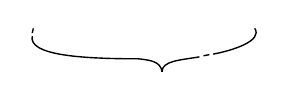
\begin{tikzpicture}[x=1em,y=1em,baseline=0pt]\draw[line width=.5pt] (0,.65) -- (-.04,.48);\draw[line width=.5pt] (-.04,.37) .. controls (-.18,-.3) and (1.6,-.45) .. (3.8,-.45) .. controls (4.25,-.5) and (4.6,-.55) .. (4.65,-.92);\draw[line width=.5pt] (8,.65) .. controls (8.3,.2) and (7.2,-.15) .. (6.5,-.28);\draw[line width=.5pt] (6.36,-.3) -- (6.15,-.34);\draw[line width=.5pt] (6,-.38) .. controls (5.3,-.5) and (4.65,-.52) .. (4.65,-.92);\end{tikzpicture}\end{tabular} transformant isomo\unsure{r}phismes en isomorphismes) correspondent aux faisceaux localement constant
i.e. les objets localement constants de $\widetilde C$, définis intrinsèquement en te\unsure{r}
de $\widetilde C$. Ainsi, le fait pour un foncteur $F:C\longrightarrow C'$ d'induire un\deleted{e \unsure{équivalence}}
homotopisme $S(C)\longrightarrow S(C')$ ne dépend que du morphisme de topos $\widetilde F:\widetilde C\longrightarrow\widetilde C'$
induit, et signifie que pour tout faisceau localement constant $F'$ sur $C'$
\unsure{c.|e.} sur $\widetilde C'$, les applic\unsure{a}tions induites $H^i(\widetilde C',F')\longrightarrow H^i(\widetilde C,\widetilde F^*.(F'))$
sont des isomorphismes (pour les $i$ pour lesquels cela a un\deleted{e\unsure{n|m}} sens).

\margin{2}

\cotefile{162-5}
\scanpage{4}
\mspage{\handwritten{2}}

On a aussi un foncteur évident
\[ T:(\mathrm{Ssimpl})\longrightarrow(\mathrm{Cat}), \]
en associant à tout ensemble semi-simplicial $X$ la catégorie $T(X)=\handwritten{\Delta}_{/X}$
des simplexes sur $X$, dont l'ensemble des objets est la réunion d\unsure{\deleted{c}i|\deleted{i}c}sjointe
des $X_n$ .... (c'est une catégorie fibrée sur la catégorie $\handwritten{\Delta}$ des simplexes
types, à fibres les catégories discrètes définies par les $X_n$). Ceci posé
Quillen prouve que pour tout $X$, $ST(X)$ est isomorphe canoniquement à $X$ da
la catégorie homotopique construite avec (Ssimpl), et que pour toute $C$,
la catégorie $TS(C)$ est \begin{tabular}[b]{@{}l@{}}\inserted{canoniquement}\\[-.55ex]\begin{tikzpicture}[x=1em,y=1em,baseline=0pt]\draw[line width=.45pt] (0,-.7) -- (0,-.35);\draw[line width=.45pt] (.03,-.23) .. controls (.1,.2) and (.35,.38) .. (.6,.4);\draw[line width=.45pt] (.7,.41)--(1.4,.41);\draw[line width=.45pt] (1.5,.4) .. controls (3,.08) and (4,.45) .. (5.4,.15) .. controls (6.4,-.05) and (7.6,-.2) .. (8.2,.1) -- (8.2,.95);\end{tikzpicture}\end{tabular} ``homotopiquement équivalente à $C$'' \deleted{dans le sens} i.e
\inserted{\unsure{c|è}a\unsure{n|a}oniquement} isomorphe à $C$ dans la catégorie quotient de (Cat) obtenue en inversant le
foncteurs qui sont des homotopismes. \deleted{Il en résulte} Ces isomorphismes son
fonctoriels en $X$. I\rlap{\begin{tikzpicture}[x=1em,y=1em,baseline=0pt]\draw[line width=.045em] (.02,.95)--(.36,.95);\draw[line width=.045em] (.18,.02)--(.18,-.19);\end{tikzpicture}}l en résulte formellement qu'un morphisme $f:X\longrightarrow Y$ dans
(Ssimpl) est un homotopisme si et seulement si il en est ainsi de $T(f):T($
$\longrightarrow T(Y)$, d'où des foncteurs $S':(\mathrm{Cat})'\longrightarrow(\mathrm{Ssimpl})'$ et $T':(\mathrm{Ssimpl})'\longrightarrow(\mathrm{C}$
entre les catégories ``homotopiques'', \begin{tabular}[b]{@{}l@{}}\inserted{construites avec (Cat) resp.(Ssimpl),}\\[-.7ex]\begin{tikzpicture}[x=1em,y=1em,baseline=0pt]\draw[line width=.45pt] (.5,.5) .. controls (-.05,.4) and (-.15,-.1) .. (.1,-.7);\draw[line width=.45pt] (16,.15) .. controls (16.25,.4) and (16.45,.62) .. (16.5,.9);\end{tikzpicture}\end{tabular} qui sont quasi-inverses l'un de l'au
re.

\deleted{d}De plus, Quillen construit un isomorphisme canonique et fonctoriel
dans (Cat)' entre $C$ et la catégorie opposée $C^{o}$, ou ce qui revient au
même, un isomorphisme canonique et fonctoriel dans (Ssimpl)' entre $S(C)$ e
$S(C^{o})$. \deleted{Cela lui permet alors, pour} La définition est telle que le
foncteur induit sur les systèmes locaux sur $C$ trahs\unsure{\deleted{o}f|\deleted{f}o}\unsure{\deleted{f}o|\deleted{o}f}rme le foncteur
contravariant $F$ sur $C$, transformant toute flêche en flêche inversible, en
le foncteur covariant (i.e. contravariant sur $C^{o}$) ayant mêmes valeurs sur
les objets, et obtenu sur les flêches en remplaçant $F(u)$ par $F(u)^{-1}$; en
d'autres termes, l'effet de l'homotopisme de Quillen sur les group\unsure{\deleted{i}o|\deleted{o}i}ides
fondamentaux est l'isomorphisme évident entre les groupoides fondamentaux
de $C$ et de $C^{o}$, \deleted{qui est l'id \unsure{en|em}} compte tenu que le deuxième est l'opposé d\unsure{u}

\margin{\handwritten{3}}

\scanpage{5}
\mspage{3}

premier. Comme application, Quillen obtient une interprétation faisceau\illegible{1}
que de la cohomologie d'un ensemble semi-simplicial à coéfficients dans \illegible{1}
système \begin{tabular}[b]{@{}l@{}}\inserted{\uline{local}}\\[-.65ex]\begin{tikzpicture}[x=1em,y=1em,baseline=0pt,line width=.45pt]\draw (2.8,.75) .. controls (3.1,.05) and (.4,-.05) .. (0,-.8);\end{tikzpicture}\end{tabular} con\deleted{tra}variant \begin{tabular}[b]{@{}l@{}}\inserted{$F$}\\[-.65ex]\begin{tikzpicture}[x=1em,y=1em,baseline=0pt,line width=.45pt]\draw (-.1,-.4)--(.8,.7);\end{tikzpicture}\end{tabular} d\deleted{\unsure{e}}(défini classiquement par le complexe cosimplici\unsure{a}
\margin{$\Pi$ ?} des $C^n(F) = \coprod_{x\unsure{\in|:}X_n} F(x)$ ): on considère le système local contravariant
défini par F, on l'interprète comme un faisceau sur \begin{tabular}[b]{@{}l@{}}\inserted{$T(X)$ i.e. objet de}\\[-.65ex]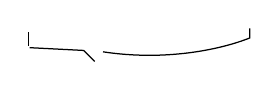
\begin{tikzpicture}[x=1em,y=1em,baseline=0pt,line width=.45pt]\draw (0,.25)--(0,-.25);\draw (.05,-.3)--(2,-.4)--(2.4,-.8);\draw (2.7,-.45) .. controls (5,-.8) and (7,-.35) .. (8,.05)--(8,.4);\end{tikzpicture}\end{tabular} $(\mathrm{Ssimpl})_{/X}$ , et on
prend sa cohomologie. - Cependant, quand F est un système de coéfficien\unsure{\deleted{s}t|\deleted{t}s}\illegible{1}
\margin{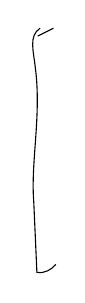
\begin{tikzpicture}[x=1mm,y=1mm]\draw (1,31) .. controls (-0.5,30) and (0.2,28) .. (0.4,26) .. controls (1.2,20) and (-0.2,14) .. (0.2,9) -- (0.6,0) .. controls (1.6,-0.2) and (2.5,0.4) .. (3,1); \draw (0.7,30) -- (2.7,31); \end{tikzpicture}}
covariant pas nécessairement local, on n'a tjrs pas d'interp\unsure{\deleted{é}r|\deleted{r}é}étation de \illegible{1}
\margin{Si !} groupes de cohomologie classiques en t ermes faiscdautiques; ni, lorsque
est \unsure{contravariant|contravatiant}, de son homologie, ou inversement de sa cohomologie
faisceautique en termes classiques.

A propos de la notion de foncteur qui est un homotopisme. Quillen
\margin{\begin{tikzpicture}[x=1mm,y=1mm]\draw[line width=.2pt] (0.5,30) -- (0.3,28); \draw[line width=.2pt,densely dashed] (0.3,28) .. controls (-0.1,20) and (0.1,7) .. (0.6,0); \draw[line width=.2pt,densely dashed] (1.2,19) -- (1.4,10); \draw[line width=.2pt] (1.4,10) -- (1.6,9.5) -- (2.3,9.4); \draw[line width=.2pt,densely dashed] (1.5,8.7) -- (2,0); \end{tikzpicture}}
montre qu\deleted{e}'un tel foncteur $F\colon C \to C'$ induit une équivalence entre la sou
catégorie triangulée \begin{tabular}[b]{@{}l@{}}\inserted{$D^b_{lc}(C')$}\\[-.65ex]\begin{tikzpicture}[x=1em,y=1em,baseline=0pt,line width=.45pt]\draw (0,-.7) .. controls (-.2,-.2) and (.15,.2) .. (.3,.05);\draw (.4,-.05)--(1.2,-.05);\draw (1.3,-.05) .. controls (3,.05) and (4.7,.5) .. (5,.85)--(4.9,1);\end{tikzpicture}\end{tabular} de la catégorie \inserted{dérivée \inserted{bornée} de celle \deleted{des}} des faisceaux abéliens sur C', don
les faisceaux de cohomologie sont des systèmes locaux, et la catégorie a\illegible{1}
logue pour C; \deleted{\unsure{Il s'en|Il en}} et réciproquement. \deleted{Pour la partie directe} On peut
dans cet énoncé introduire aussi n'importe quel anneau de base (à conditi
de le supposer $\neq 0$ dans le cas de la réciproque); \deleted{constant} la partie dir
vaut aussi avec un anneau de boefficients pas néc. constant, mais consta
tordu. Je pense que ce résultat (facile) doit pouvoir se généraliser ai
Soit $f\colon X \quad X'$ un morphisme de topos qui soit tel que pour tout \deleted{syst\unsure{è|ê}}
faisceau loc. const. sur X', f induise un isomorphisme sur les cohomolog
(avec cas non commutatif inclus). Supposons que \deleted{$\unsure{X|F}$ (resp. $\unsure{X|X'}$)} \inserted{\unsure{X} et X'} \unsure{\deleted{soi}t|soit} \uline{locale}
\margin{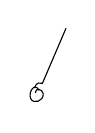
\begin{tikzpicture}[x=1mm,y=1mm]\draw (1.1,1.5) .. controls (0.5,2.6) and (-0.3,1.3) .. (0,0.5) .. controls (0.3,-0.3) and (1.7,0.1) .. (1.6,1.1) .. controls (1.5,1.7) and (0.6,1.9) .. (0.6,1.2); \draw (0.5,1.8) .. controls (0.8,2.7) and (1.2,2.4) .. (1.5,2.4) -- (4.5,9.4); \end{tikzpicture}}
\margin{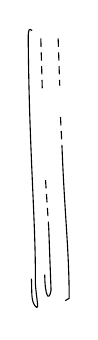
\begin{tikzpicture}[x=1mm,y=1mm]\draw (0.5,35) .. controls (0.1,35.3) and (0,35.2) .. (0,34) .. controls (0.1,20) and (1,10) .. (0.9,3) .. controls (1,1) and (1.5,-0.7) .. (0.9,0) .. controls (0.3,0.7) and (0.5,2) .. (0.4,3.5); \draw[densely dashed] (1.6,34) -- (1.8,27); \draw[densely dashed] (2.2,16) -- (2.6,10); \draw (2.6,10) -- (2.9,2) .. controls (2.6,0.4) and (2.1,1.5) .. (2.1,4); \draw[densely dashed] (3.8,34) -- (4,28); \draw[densely dashed] (4.1,24) -- (4.3,20); \draw (4.3,20) .. controls (4.6,12) and (5.2,7) .. (5.2,1) -- (4.7,0.7); \end{tikzpicture}}
\uline{homotopiquement trivial}, i.e. que \deleted{tout} pour tout entier n \begin{tabular}[b]{@{}l@{}}\inserted{$\geq 1$}\\[-.65ex]\begin{tikzpicture}[x=1em,y=1em,baseline=0pt,line width=.45pt]\draw (0,-.8) .. controls (.2,.1) and (1.6,.15) .. (1.8,.8)--(1.8,1);\end{tikzpicture}\end{tabular}, tout objet U \illegible{1}
\deleted{\unsure{X'|U'}} ait un \deleted{rev\unsure{ê}tement} \inserted{recouvrement} par des $U_i \to U$, tels que a) tout systême local sur
devient constant sur $U_i$ , et toute section sur U devient constante sur U
et b) pour tout \deleted{systême} groupe abélien G, les $H^j(U,G) \longrightarrow H^j(U_i,G)$ son
nuls pour $1 \leq j \leq n$. Alors le foncteur $D^b_{lc}(X') \longrightarrow D^b_{lc}(X)$ induit par f est

\noindent\begin{tikzpicture}[x=1cm,y=1cm,line width=0.3pt]
\draw (0,0)--(.08,.01);\draw (.12,.02) .. controls (.4,.06) and (.7,.04) .. (.9,.08)--(1.25,.12);\draw (1.29,.12)--(1.62,.15);\draw (1.67,.15)--(1.8,.16);\draw (1.84,.17)--(1.96,.18);\draw (2.1,.19)--(2.48,.22);\draw (2.53,.22)--(2.72,.23);\draw (2.78,.23)--(2.88,.23);\draw (3,.22) .. controls (3.3,.15) and (3.6,.14) .. (3.9,.13);\draw[densely dashed] (3.92,.13)--(4.35,.1);\draw (4.4,.1)--(4.75,.1);\draw[dotted] (5.9,.1)--(6.1,.1);\draw[densely dashed] (6.8,.06)--(7.1,.01);\draw[dotted] (7.15,.01)--(7.45,.02);\draw[densely dashed] (7.5,.03)--(7.9,.04);\draw[dotted] (7.95,.04)--(8.2,.05);\draw[densely dashed] (8.6,.07)--(8.95,.09);\draw[dotted] (9,.09)--(9.3,.1);\draw[densely dashed] (9.6,.12)--(10.2,.12);\draw[dotted] (10.25,.12)--(10.75,.11);\draw[densely dashed] (11.1,.11)--(11.6,.12);\draw (11.65,.12)--(11.83,.12);\draw[densely dashed] (11.88,.12)--(12.4,.12);\draw (12.45,.12)--(13.2,.1);
\end{tikzpicture}

\margin{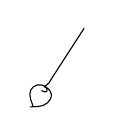
\begin{tikzpicture}[x=1mm,y=1mm]\draw (0.1,0).. controls (0.6,0.1) and (1.7,-0.1)..(2.3,0.5).. controls (3.3,1.4) and (2.7,2.2)..(2.2,2.5).. controls (1.4,3.1) and (0.5,2.8)..(0.2,2.1).. controls (-0.1,1.3) and (0.4,0.6)..(0.5,0.1); \draw (1.6,2.1).. controls (2.3,1.6) and (2.5,2.2)..(2.1,2.5); \draw (1.9,2.5).. controls (2.2,2.9) and (2.5,2.8)..(2.8,3.5) -- (7,10); \end{tikzpicture}}
\handwritten{Attention, cette condition n'est typiquement \uline{pas} satisfaite par les schémas a
leur \unsure{topologie} \unsure{étale} (mais bien \unsure{sur|par} \unsure{schémas|variétés} \unsure{l.}noeth. avec top. Zariski).}

\margin{4}

\scanpage{6}
\mspage{\handwritten{4}}

\deleted{pleinement fidèle (resp} une équivalence). Même énoncé si on met dans le
coup un \deleted{Anneau loc} systême local d'anneaux sur X'. Enfin, f induit \deleted{un}
\inserted{\deleted{foncteur \unsure{soit équiv.|plein fid} (resp} une équivalence).}
\deleted{isomorphisme} entre la catégorie des coefficients locaux sur C et celle
des coéff. locaux sur C' \deleted{(?? peut être}
\inserted{\deleted{cette propriété doit}}
\deleted{\unsure{il|l} doit il être \unsure{mise|mis} dans les
hypothèses préliminaires sur f ?)} Principe de démonstration: on commence
par prouver ce dernier résultat, en notant que \deleted{dans le ca} si un topos est
localement hom. trivial, il est loca connexe et loc. simplement connexe,
d'où une bonne théorie du $\handwritten{\pi}_{0}$ et du $\handwritten{\pi}_{1}$ (qui sont ici discrets), et on est
ramené \deleted{pour} à un cas particulier du critère d'homotopisme de Artin et
Mazur, savoir un critère \begin{tabular}[b]{@{}l@{}}\inserted{cohomologique}\\[-.6ex]\begin{tikzpicture}[x=1cm,y=1cm,baseline] \draw (0,0) .. controls (-.17,.15) and (-.12,.43) .. (.13,.64); \draw (.18,.69) .. controls (.55,.95) and (1.08,.96) .. (1.55,.87) .. controls (1.92,.8) and (2.17,.81) .. (2.35,.8); \draw[dotted] (2.43,.8) -- (3.42,.84); \draw (3.51,.85) -- (3.73,.88); \draw[dotted] (3.77,.9) -- (3.94,1.02); \draw (3.99,1.08) .. controls (4.04,1.25) and (4.03,1.37) .. (3.94,1.45); \end{tikzpicture}\end{tabular} pour qu'un homomorhisme de groupes $G\handwritten{\to} H$ (ici de
groupes $\handwritten{\pi}_{1}$ de X,X') soit un isomorphisme: il doit induire des isomorphismes sur les $H^{o}$ et $H^{1}$ (y inclus dans le cas non commutatif...). On prouve
la pleine fidélité en se ramenant par la suite spectrale aux cas des $\mathrm{Ext}^{\unsure{i}}$
de coéfficients locaux. Par la suite spectrale encore, cela résultera du
fait suivant: si X\deleted{'} est \unsure{\deleted{l}h|\deleted{h}l}omalement hom. trivial, alors la catégorie des
faisceaux abéliens loc. constants est stable par $\underline{\mathrm{Ext}}^{i}$ , et le foncteur
$M\handwritten{\mapsto} M_{X}$ \deleted{des fai\unsure{sce}a\unsure{ux} constants} (Ab) dans $X_{ab}$ commute aux dits $\mathrm{Ext}^{i}$ .
En fait, X et X' étant loc.homp\begin{tikzpicture}[x=1cm,y=1cm,baseline=0pt]\draw[line width=.4pt] (0,.35)--(-.08,.85);\draw[line width=.4pt] (.02,-.08)--(.1,-.65);\end{tikzpicture}triviaux, les conditions suivantes sur f
seront équivalentes:

a) f est\unsure{!)|\deleted{'}} un homotopisme, i.e. induit pour tout systême local (pas
néc commutatif) sur X'un isomorphisme sur les $H^{i}$\deleted{pour i \unsure{m}}.

b) \deleted{Même chose ave} f induit une équivalence $D^{b}_{lc}(X')\handwritten{\longrightarrow} D^{b}_{lc}(X)$ .

a\handwritten{'}) f induit une équivalence entre la catégorie des systêmes locaux
abéliens sur X' et X, et des isomorphismes sur les $H^{\unsure{i|1}}$ correspondants (do\unsure{n}
on ne prend ici que des coéfficients commutatifs).

\margin{\handwritten{?}} J'ignore si on peut dans a) se borner aux systêmes locaux commutatif\unsure{s}

\deleted{i e \unsure{dan}}
L'équivalence entre a) et b) fournit une première justification ou
motivation pour définir des types d'homotopie via la catégorie $D\handwritten{^{b}_{lc}(X)}$,

\margin{\handwritten{5}}

\scanpage{7}
\mspage{5}

éventuellement muni de la sous-catégorie pleine de tous les systêmes loc
sur X, et du foncteur cohomologique sur $D^{b}_{lc}(X)$ à valeurs dqns laddt\unsure{ë}
catégorie, et bien sûr du produit tensoriel (mais alors on sort de $D^{b}$
pour entrer dans $D^{-}$ , redactor demerdetur).

II \quad $n$-catégories, catégories $n$-uples, et (Gr)-catégories.

Appelons bi-catégorie une catégorie dans(Cat), i.e. un triple
($C^{\deleted{o}}_{\handwritten{0}}$,$C^{\deleted{1}}_{\handwritten{1}}$, \deleted{\illegible{2}o\unsure{ï|i}}$p_{1}$,$p_{2}$, $\handwritten{\pi}$ ), où $C^{o}$ est une catégorie, $p_{1}$,$p_{2}$: $C^{\deleted{1}}_{\handwritten{1}} \handwritten{\rightrightarrows} C^{\deleted{o}}_{\handwritten{0}}$ deux
foncteurs, $\handwritten{\pi}$:$(C^{\deleted{1}}_{\handwritten{1}},p_{1})\mathrm{x}_{C^{o}}(C^{\deleted{1}}_{\handwritten{1}},p_{2}) \handwritten{\longrightarrow} C^{\deleted{1}}_{\handwritten{1}}$ un foncteur, avec les axiomes
habituels. Interprétant (Cat) comme la sous-catégorie pleine de (Ssimpl
des objets qui .... , et de même pour les catégories à valeurs dans une
catégorie telle (Cat), on trouve que la catégorie \inserted{(Bicat)} des (Cat)-catégories
est équivalente à la sous-catégorie pleine de la catégorie des ensembles
bi-semisimpliciaux

\[
\begin{array}{cccc}
X^{\deleted{00}}_{\handwritten{00}} & X^{\deleted{01}}_{\handwritten{01}} & \ldots & X^{\deleted{0n}}_{\handwritten{0n}}\\
X^{\deleted{10}}_{\handwritten{10}} & X^{\deleted{11}}_{\handwritten{11}} & \ldots & X^{\deleted{1n}}_{\handwritten{1n}}\\
\multicolumn{2}{l}{.\,.\,.\,.\,.\,.\,.} & &
\end{array}
\]

formée des objets qui ligne par ligne et colonne par colonne satisfoht la
condition d'exctitude familière (transformer sommes amalgamées en produi\unsure{t}
fibrés). De même la catégorie \deleted{des} (Tricat) des (Bicat)-catégories
\unsure{\deleted{'}s|\deleted{s}'}\unsure{\deleted{s}'|\deleted{'}s}interprète en t ermes d'objets tri-\begin{tabular}[b]{@{}l@{}}\inserted{semi}\\[-.6ex]\begin{tikzpicture}[x=.65cm,y=.4cm,baseline=0pt]\draw[line width=.5pt] (0,-.35)..controls(.25,.2)and(.5,.45)..(.8,.5)--(1.1,.53);\draw[line width=.5pt] (1.22,.57)..controls(1.55,.75)and(2.1,.7)..(2.3,.95)..controls(2.38,1.04)and(2.35,1.16)..(2.3,1.25);\end{tikzpicture}\end{tabular}simpliciaux, etc.

Exemple: soit C une catégorie, posons $C^{\deleted{o}}_{\handwritten{0}}$=C, $C^{\deleted{1}}_{\handwritten{1}}$=$\underline{Fl}$(C), avec structure
$p_{1}$,$p_{2}$, évidentes (d'où une (Cat)-catétorie dont les composantes semi-si\unsure{m}pliciales supérieures sont les catégories $\underline{Fl}^{n}$(C) des $n$-flêches de C ...)
L'ensemble bi-semisimplicial correspondant a pour composantes les ensembl
Hom($\handwritten{\Delta}^{n}\handwritten{\unsure{\times|\alpha}}\handwritten{\Delta}^{m}$,C). Par exemple, les objets de $X^{\deleted{11}}_{\handwritten{11}}$ sont les carrés commutatif
de flêches de C, qu'on peut interpréter(de deux manières différentes) co\unsure{m}

\margin{6}

\scanpage{8}
\mspage{6}

morphismes de flêches.

Notons une symmétrie évidente dans la \unsure{catégorie|c atégorie} (Bicat), interprété
en termes d\deleted{\unsure{a|e}}'ensemble bi-semisimpliciaux, obtenue en échangeant les lign
et les colonnes dqns \deleted{les} de tels ensembles bi... \unsure{\deleted{q}U|\deleted{U}q}n ensemble bisemisimpl
al qui ... peut donc de deux façons différentes être consi\deleted{i}déré comme déf
nissant une bicatégorie. De même le groupe symétrique $\mathrm{Sym}_n$ opère sur
la catégorie \deleted{de} (\unsure{nupcat|n-upcat}) des catégories n-uples ..

Une 2-catégorie peut être définie comme constituée par un ensemble
\deleted{discret} $C^{\deleted{\unsure{o}}}_0$ (l'ensemble des objets ), qu'on interprètera comme une catégo%
rie discrète, plus la donnée pour tout $x,y \in \unsure{C^o_0}$ d'une catégorie $\underline{\mathrm{Hom}}(x,y)$,
plus \deleted{une} \inserted{des foncteurs} composition entre celles\unsure{\deleted{(}-|\deleted{-}(}ci ... Prenant la catégorie somme \deleted{de} C
des $\underline{\mathrm{Hom}}(x,y)$, On peut exprimer la donnée de ces foncteurs de composition
et des sources et buts\begin{tabular}[b]{@{}l@{}}\inserted{$x,y\unsure{)}$}\\[-.6ex]\begin{tikzpicture}[x=1mm,y=1mm,baseline=0pt]\draw[line width=.5pt] (0,0)..controls(2,1.6)and(4.7,3.2)..(6.8,4.2);\draw[line width=.3pt] (7.1,4.4)--(7.5,4.7);\draw[line width=.3pt] (7.7,4.9)--(8.4,5.7);\draw[line width=.3pt] (8.6,5.9)--(9,6.5);\end{tikzpicture}\end{tabular} dans les catégories $\underline{\unsure{\deleted{P}H|\deleted{R}H|\deleted{H}P|\deleted{H}R}\mathrm{om}}(x,y)$, comme définis par
des foncteurs ``source'' et ``but'' $C^{\deleted{1}}_1 \to \unsure{C^o_0}$, et un foncteur de composition
$C^{\deleted{1}}_1 \mathrm{x}_{C^o_0} C^{\deleted{1}}_1 \longrightarrow \unsure{C^{\deleted{1}}_1}$ , les axiomes des 2-catégories correspondant exactement au
axiomes des(Cat)-catégories. De cette façon, la catégorie des 2-catégor
est équivalente à la catégorie des (Cat)-catégories qui ont une ``catégo
d'objets'' qui est discrète, ou encore à la catégorie des Bicatégories
qui, interprétées comme ensembles bi-semisimpliciaux, ont \deleted{une} comme
première ligne un ensemble bemis\unsure{\deleted{s}i|\deleted{i}s}\unsure{\deleted{i}m|\deleted{m}i}plicial discret (i.e. un foncteur cons%
tant sur $\Delta$ ). Il parait qu'on a une interprétation simple dans le même
esprit de la notion de n-catégorie en termes d'ensembles n-semi-simplici
\margin{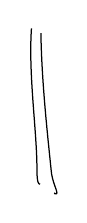
\begin{tikzpicture}[x=1mm,y=1mm]\draw[line width=.45pt] (0,21).. controls (-0.4,15) and (0.7,8)..(0.7,3).. controls (0.7,1.4) and (0.9,1.2)..(1.1,1.2); \draw[line width=.45pt] (1.2,20.4).. controls (1.3,14) and (2.1,7)..(2.5,3).. controls (2.6,1.5) and (3.4,0.2)..(3.2,0).. controls (3.1,-0.1) and (2.9,0)..(2.9,0.1); \end{tikzpicture}}
\deleted{\unsure{ou|au}} Demander à Quillen relations entre la notion de m-Catégorie dans
la catégorie (n-Cat), et celle d\deleted{\illegible{1}}\inserted{'} ensemble (m+n)-semisimplicial.
\deleted{(en particulier entre cette dernière notion et celle de}

L'interprétation standard semisimpliciale permet d'interpréter

\margin{7}

\scanpage{9}
\mspage{7}

\noindent
\begin{minipage}{.06\linewidth}
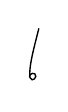
\begin{tikzpicture}[x=1em,y=1em]
\draw[line width=.5pt] (.5,2.1) .. controls (.35,1.5) and (.12,.7) .. (.18,.32)
 .. controls (.25,.12) and (.48,.35) .. (.35,.46)
 .. controls (.23,.52) and (.12,.38) .. (.18,.32);
\end{tikzpicture}
\end{minipage}
\begin{minipage}{.9\linewidth}
\begin{tabular}{|p{.94\linewidth}|}
\handwritten{Attention : la catégorie $\underline{\mathrm{Hom}}_{\mathrm{gr-b}}$, qui s'identifie à la catégorie définie
par un $\unsure{R|\mathbb{R}}\mathrm{Hom}_{\mathbb{Z}}(C_{\unsure{x|\bullet}}, C'_{\unsure{x|\bullet}})$; ce point devant être élucidé !}\\
\hline
\end{tabular}
\end{minipage}

de même les (Cat)-groupes(ou groupes à valeurs dans (Cat)) comme étant
les groupes semisimpliciaux qui ``sont''des catégories i.c. qui \deleted{se défini\unsure{s|d}}
\deleted{sent} sat\unsure{\deleted{s}i\deleted{i}s|\deleted{i}s\deleted{s}i}font la condition d'exactitude familière, permettant d'en déte
miner tous les composants à l'aide de $C_{o\deleted{a}}$ et $C_1$ . Appliquant le tapis de
Dold, dans le cas commutatif, on trouve que les (Cat)-groupes abéliens
forment une catégorie équivalente à celle des complexes de chaines de
groupes abéliens qui sont de longueur 1:
\[ 0 \leftarrow C_o \leftharpoonup C_1 \leftarrow 0 \quad . \]
Quand on explicite la (Cat)-groupe abélien associé à un tel complexe de
chaines, on trouve ``ma'' construction chérie da la ``catégorie de Picard''
associée au complexe: objets ceux de $C_o$ , flêches de x dans y les z dans
tels que $dz = y-x$ . On trouve donc à isomorphisme ppès tous les group\unsure{e}
abéliens de (Cat) ainsi. Un complément important est que toute catégori
\margin{\handwritten{\deleted{\unsure{Objection déjà}, mais cela contredit les \unsure{résultats} de \illegible{2 lignes}}}}
de Picard \deleted{\inserted{(resp. et} commutative)}est équivalente (au sens technique qu'on ne précis
pas ici) à \deleted{la catégorie} un vrai (Cat)-groupe \deleted{\inserted{(resp. (Cat)-groupe} commutatif)}\begin{tikzpicture}[x=1cm,y=1cm,baseline=0pt]\draw[line width=.45pt] (0,.7)--(.01,.5);\draw[line width=.45pt] (.03,.43)..controls(.1,.29)and(.3,.29)..(.5,.32);\draw[line width=.45pt] (.75,.2)..controls(.63,.02)and(.59,-.16)..(.61,-.35);\end{tikzpicture} .
\inserted{\handwritten{Quand on
\unsure{identifie|simplifie} mod ``\unsure{Gros|Grab}'' équivalence, cela correspond à travailler dans la catégorie \uline{déri\unsure{v}}
des complexes, seuls invariants \unsure{étant|sont} $\pi_o, \pi_1$)}}
\margin{\handwritten{\unsure{Mais} \unsure{si on part} d'une ``cat. de Picard \unsure{commut.}'' elle \unsure{ne se réalise} que par un $(\mathrm{Cat})$-g. \uline{\uline{\unsure{non}}} \uline{\unsure{comm.}}}}
On notera qu'on a une \deleted{\unsure{l|t}\illegible{5}} classification beaucoup plus restrein
que pour les H-espaces (resp. les H-espaces homotopiquement comm.) mod
équivalence d'homotopie, de façon précise entre les groupes resp. les gr
oupes abéliens de la catégorie homotopique. La raison en est qu\inserted{\handwritten{'}}on est beau
coup plus restrictif dans le contexte catégorique pour le sens d\unsure{a|e} l'asso\unsure{c}
tivité (resp. et de la commutativité), puisqu'on ne demande pas seulemen\unsure{t}
l'existence d'isomorphismes d'associ\unsure{\deleted{t}a|\deleted{a}t}itivité\deleted{\unsure{,}} (qui suffirait pour avoir \unsure{u}
groupe dans \begin{tabular}[b]{@{}l@{}}\inserted{la catégorie homotopique}\\[-.6ex]\begin{tikzpicture}[x=1cm,y=.7cm,baseline=0pt]\draw[line width=.45pt] (0,.8)..controls(-.1,.55)and(-.08,.16)..(.18,.14)..controls(.4,.13)and(.57,.23)..(.8,.18)--(1.7,.16)..controls(1.8,.15)and(1.87,.1)..(1.95,.09);\draw[line width=.45pt] (2.02,.09)..controls(2.2,.14)and(2.35,.2)..(2.5,.18)--(3.1,.15)..controls(3.4,.15)and(3.48,.03)..(3.5,-.3)..controls(3.53,-.05)and(3.57,.13)..(3.8,.12);\end{tikzpicture}\end{tabular} $(\mathrm{Cat})' \mathrel{\underline{\approx}} (\mathrm{Ssimpl})'$, modulo l'existence d'unités et d'invers
mais qu'on suppose \uline{donné\deleted{e}s} ces isomorphismes, de façon à satisfaire à ce\unsure{r}
taines compatibilités: c'est ce qui permet, me semble-t-il, de prouver q\unsure{u}
\margin{\handwritten{\deleted{\uuline{\unsure{pourquoi}}}}}
\margin{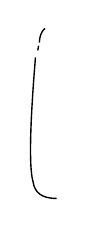
\begin{tikzpicture}[x=1cm,y=1cm,baseline] \draw[line width=.5pt] (.15,2.2) .. controls (.1,2.16) and (.08,2.08) .. (.08,2.02); \draw[line width=.5pt] (.07,1.98) -- (.06,1.92); \draw[line width=.5pt] (.03,1.83) .. controls (-.03,1.1) and (-.06,.45) .. (0,.25) .. controls (.02,.12) and (.1,.04) .. (.3,.04); \end{tikzpicture}}
équivalence près, on peut supposer qu'il s'agit de vrais groupes dans
(Cat), \deleted{resp. de vraie commutativité.}

\margin{\handwritten{8}}

\scanpage{10}
\mspage{\handwritten{\shortstack{\tikz[scale=.2]{\draw (0,0) .. controls (.2,.12) and (.4,.12) .. (.6,0);}\\8}}}

On doit trouver une approximation meilleure d'un cran à la classifi
tion topologique en prenant des (2-Cat)-groupes resp. des (2-Cat)-group
abéliens, ou plus généralement des `` Gr-2'-catégories '' resp.
``G\unsure{\deleted{n}r|\deleted{r}n}ab-2-catégories'' . (NB U\unsure{\deleted{n}n}e Grab-catégorie défi\deleted{\unsure{i|k}}nit une Grab-2catégor
comme une catégorie définit une 2-catégorie; du point de vue semi-simpli
al, cette opération serait analogue à celle de ``cosquélette$^{\text{x}}$ tronqué'';
Mais également une Grab-2-catégorie défini$\overset{\handwritten{\text{t}}}{\text{e}}$ $\overset{\handwritten{\text{une}}}{\text{en}}$ G\unsure{\deleted{R}r|\deleted{r}R}ab-catégorie$^{\text{x}}$, savoir la
catégorie des automorphismes de l'objet unité; cette \deleted{dé} opération serait
analogue à celle de ``tuage des groupes d'homotopie en dim $\handwritten{>}\unsure{\deleted{2}\handwritten{1}}$''). Pour l
notion gro\deleted{i}ssière ( Gra\deleted{b} ou Grab) l'idée de ma lettre à Verdier était qu
doit trouver la même chose que les tronqués \inserted{au cran 2}, dans la catégorie \uline{homotopi\unsure{q|c}}
des H-espaces - i.e. ce qu'on déduit des H-espaces par tuage des group
d'homotopie en dimensions $\handwritten{>}2$ .

\margin{\handwritten{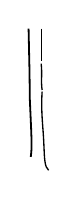
\begin{tikzpicture}[x=1mm,y=1mm]\draw[line width=.65pt] (0,18)--(.05,15.7)--(.12,12.5)--(.16,9)--(.32,5.4)..controls(.4,3.5)and(.4,2.5)..(.28,1.7);\draw[line width=.48pt] (1.6,18)--(1.6,13.85);\draw[line width=.48pt] (1.6,13.55)..controls(1.75,12.2)and(1.55,11.3)..(1.72,10.2);\draw[line width=.48pt] (1.72,10.0)..controls(1.55,7.3)and(1.85,5.7)..(1.95,3.1)..controls(2.02,1.6)and(2.02,.4)..(2.55,0);\end{tikzpicture}}}
(Demander à Quillen relations exactes entre \deleted{H}objets-groupes et objet
\inserted{\deleted{ponctués}}connexes de la catégorie homotopique\inserted{ponctuée}: forment-ils des catégories équival
tes par le foncteur espace des lacets\handwritten{?}).
\margin{\handwritten{non, on a\\un foncteur\\\unsure{pl.} fidèle (?)\\\unsure{mais} \unsure{pas} \unsure{ess.}\textsuperscript{t}\\surjectif....}}

Pour les \uline{vrais} groupes \inserted{abéliens} de (2-\unsure{\deleted{C}C|\deleted{o}C|\deleted{C}o}at), l'approche de Quillen consiste à
les identifier à'abord à des groupes abéliens de la catégorie \deleted{t}\handwritten{(}Bicat),
donc à des grpupes abéliens bi-semiesimpliciaux particuliers (conditions
sur chaque ligne et chaque colonne). Appliquant la version bi-semisimpli
ale du tapis de Dold, on trouve que \deleted{c\unsure{e}tt\unsure{e} c\unsure{a}} la catégorie de ces objets
esth équivalente à la catégorie des \deleted{objets} bicomplexes \inserted{de chaines} de groupes abéli
qui sont nuls en dehors du carré $\unsure{\deleted{D}0|\deleted{0}D}\handwritten{\leq}i,j\handwritten{\leq}1$. \deleted{Quillen dit que} La \deleted{colonn}\inserted{\handwritten{cond.}}
que la première ligne corresponde à un \deleted{ensemble} groupe semisimplicial
trivial signifie alors qu'elle n'a que le terme de degré zéro, i.e. que
le bicomplexe est réduit à

\diagram{
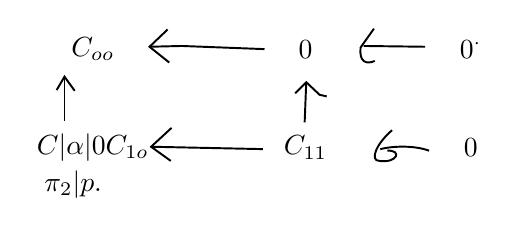
\begin{tikzpicture}[x=1cm,y=1cm,baseline=(current bounding box.center)]\node (a) at (0,1.25) {$C_{oo}$};\node (b) at (2.7,1.25) {$0$};\node (c) at (4.8,1.25) {$\handwritten{0}^{\unsure{\cdot}}$};\node (d) at (0,0) {$\handwritten{\unsure{C|\alpha|0}}C_{1o}$};\node (e) at (2.7,0) {$C_{11}$};\node (f) at (4.8,0) {$\handwritten{0}$};\node at (-.25,-.47) {$\unsure{\pi_{\unsure{2}}|p.}$};\draw[line width=.7pt] (2.18,1.25)--(1.13,1.29)--(.72,1.28);\draw[line width=.7pt] (.95,1.50)--(.72,1.28)--(.97,1.08);\draw[line width=.7pt] (4.22,1.28)--(3.44,1.29);\draw[line width=.7pt] (3.57,1.51)--(3.40,1.27)..controls(3.38,1.09)and(3.47,1.05)..(3.58,1.10);\draw[line width=.7pt] (2.16,-.02)--(.75,.01);\draw[line width=.7pt] (1.00,.25)--(.74,.01)--(.99,-.17);\draw[line width=.7pt] (4.27,-.04)..controls(4.08,.03)and(3.81,.02)..(3.65,-.02);\draw[line width=.7pt] (3.80,.22)..controls(3.60,.05)and(3.51,-.17)..(3.64,-.17)..controls(3.87,-.20)and(3.93,-.03)..(3.74,-.04);\draw[line width=.7pt] (-.36,.34)--(-.36,.90);\draw[line width=.7pt] (-.46,.73)--(-.36,.90)--(-.23,.72);\draw[line width=.7pt] (2.69,.32)--(2.71,.83);\draw[line width=.7pt] (2.57,.69)--(2.71,.83)--(2.88,.67)--(2.97,.65);\end{tikzpicture}
}
\margin{\handwritten{9}}

\scanpage{11}
\mspage{9}

\unsure{\deleted{L}C|\deleted{C}L}\unsure{\deleted{a}e|\deleted{e}a}s\deleted{\unsure{e|c}} bicomplexes s'identifient aux complexes de chhines de lo\unsure{\deleted{g}n|\deleted{n}g}gueur 2.
Donc la catégorie de (2-Cat)-groupes abéliens est équivelente à celle de
complexes de chaines de longueur 2. L'explicitation de la 2-catégorie
associée à un tel complexe de chaines est mon interprétation chérie. Il
faudrait encore expliciter les \deleted{morphismes} 2-Grab-catégorie des
homomorphismes (en un sens à préciser) entre deu\unsure{\deleted{t}x|\deleted{x}t}\deleted{\unsure{e}l} tel\unsure{\deleted{s}l|\deleted{l}s}es 2-Grab-catég
ries strictes, en termes d'un complexe RHom.

L'idée qui se dégage de cette approche, et que Quillen on espère v
expl\unsure{\deleted{o}i|\deleted{i}o}citer, c'est que la \deleted{notion de catégorie} de notion\deleted{s} de groupe \uline{abélie}
dans (n-Cat) correspond à celle de complexe de \inserted{\begin{tabular}[b]{@{}l@{}}chaines de\\[-.9ex]
\begin{tikzpicture}[x=1cm,y=1cm]\draw[line width=.45pt] (0,0)..controls(-.08,.12)and(-.02,.3)..(.20,.47)--(.24,.49);\draw[line width=.4pt] (.27,.50)..controls(.75,.61)and(1.19,.57)..(1.55,.55)--(1.70,.53)--(1.83,.54)..controls(2.05,.55)and(2.29,.57)..(2.38,.64)..controls(2.42,.68)and(2.43,.73)..(2.41,.77);\end{tikzpicture}
\end{tabular}} longueur n, en raisonnant
soit mod. isomorphisme de part et d'autre, soit mod. une notion naturell
de n-équivalence d'un côté, et dans la catégorie dérivée de l'autre. Cec
doit pouvoir se préciser en utilisant des Hom$^{\bullet}$ resp. des RHom$^{\bullet}$.

Si maintenant C est une catégorie avec un ``produit tensoriel'' assoc
tif (et éventuellement unitaire), i.e. un bifoncteur avec des isomorphis%
mes d'associativité (mais sans inverse ...), on peut lui associer \unsure{\deleted{(}s|\deleted{s}(}ans
doute une Gr-catégorie universelle (tout comme à un monoïde on associe
groupe symmétrisé), d'où des invariants, qu'on pourra désigner par K$_{o}$(C)
et K$_{1}$(C). On suppose qu'on pourra de même trouver, pour tout n, une
Gr-n-catégorie universelle où envoyer C de façon compatib\unsure{\deleted{o}l|\deleted{b}l|\deleted{l}o|\deleted{l}b}e avec $\otimes$ (\unsure{\deleted{d}t|\deleted{t}d}out
cela dans un sens à préciser), dont les invariants $\handwritten{\pi}_{n}$ seraient par déf
tion les K$_{n}$(C). \unsure{\deleted{E}U|\deleted{L}U|\deleted{t}U|\deleted{U}E|\deleted{U}L|\deleted{U}t}\unsure{\deleted{a}n|\deleted{n}a} cas intéressant est celui où C est une catégorie ave
produits finis (par exemple une catégorie additive) et $\otimes$ est le produit;
\deleted{mais}\deleted{(}\handwritten{[}\unsure{\deleted{\illegible{1}}\handwritten{M}}ais on notera que dans le cas d'une catégorie non seulement additi
mais abélienne, il y a une notion plus adéquate du K$_{o}$ , qui devrait corr
pondre à une notion plus adéquate de la suite des K$_{i}$ , inspirée du tapis
de Roos; sans doute c'est en termes de (``vraie'') catégories triangulées

\margin{10}

\scanpage{12}
\mspage{10}

qu'i\unsure{\deleted{m}l|\deleted{o}l|\deleted{l}m|\deleted{l}o} conviendra de poser les définitions adéquates). - Peut-être Quill
\margin{\handwritten{\uuline{\unsure{oui|sic}}}\figure{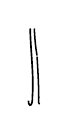
\begin{tikzpicture}[x=.035cm,y=.035cm,baseline=0pt]\draw[line width=.6pt] (0,27)..controls(.15,19)and(1.4,10)..(.8,2)..controls(.9,.4)and(.5,-1)..(-.1,-.8)..controls(-.6,-.6)and(-.6,.1)..(-.6,.8);\draw[line width=.55pt] (1.5,27)..controls(1.8,21)and(2.2,19)..(2.5,17.2);\draw[line width=.55pt] (2.5,16.8)..controls(2.8,12)and(3.2,5)..(3.1,.1)--(3.4,-.5);\end{tikzpicture}}}a-t-il une définition semi-simpliciale plus directe, sans passer par des
n-catégories, des $K_i$ et plus précisément du H-espace qui devrait correspo
dre à C. \deleted{Dans le cas} Ce n'est certainement \unsure{pas \inserted{en général} l'ensemble|\inserted{en général} pas l'ensemble} semi-simplicial
SC \deleted{engendré à} associé à C, puisque dans le cas d'une catégorie additive,
C est homotopiquement trivial (en effet le foncteur identique est ``homoto
au foncteur nul, puisqu'il suffit d'avoir un homomorphisme d'un foncteur
dans l'autre; d'où une équivalence d'homotopie entre C et la catégorie
nulle). Pourtant, il semble bien que dans le cas où C est une Gr-catégor
\margin{\figure{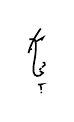
\begin{tikzpicture}[x=.04cm,y=.04cm,baseline=0pt]\draw[line width=.6pt] (1.1,11)..controls(1.7,13.8)and(3.5,16.7)..(5.0,18.8);\draw[line width=.6pt] (1.4,15.4)--(3.0,15.4)..controls(3.5,14.7)and(3.5,13.5)..(3.4,12.2)..controls(3.4,9.6)and(2.4,6.9)..(2.7,5.0)..controls(2.9,3.6)and(4.4,3.1)..(5.7,4.7)--(4.7,5.3);\draw[line width=.55pt] (3.2,14.5)--(5.8,16.0)--(5.2,15.0);\draw[line width=.5pt] (1.3,12.0)--(2.2,12.3);\draw[line width=.55pt] (5.6,8.0)--(6.2,8.0)--(6.3,7.2)--(5.4,6.5);\draw[line width=.55pt] (5.2,6.2)--(4.5,5.7);\draw[line width=.55pt] (4.1,1.0)--(5.3,1.1)--(4.8,.9)..controls(4.9,.3)and(5.4,-.1)..(5.1,-.8);\draw[line width=.7pt,line cap=round] (5.15,-1.5)--(5.18,-1.55);\end{tikzpicture}}\figure{\begin{tikzpicture}[x=.04cm,y=.04cm,baseline=0pt]\draw[line width=.6pt] (0,25)--(.7,24.9)..controls(1.1,24.7)and(.1,23.0)..(.2,22.0)..controls(.2,21.4)and(1.1,21.0)..(1.1,20.3)--(1.2,17.9);\draw[line width=.6pt] (1.2,17.2)--(1.3,16.3);\draw[line width=.3pt,opacity=.4] (1.35,15.3)--(1.4,15.0);\draw[line width=.3pt,opacity=.4,line cap=round] (1.5,12.7)--(1.5,12.6);\draw[line width=.4pt,line cap=round] (1.8,9.0)--(1.8,8.8);\draw[line width=.55pt] (2.1,6.6)--(2.2,6.2);\draw[line width=.3pt,opacity=.4] (2.5,4.0)--(2.5,3.7);\draw[line width=.6pt,line cap=round] (2.2,.2)--(2.3,.15);\end{tikzpicture}}}i.e. admet des inverses, alors ce soit bien la construction ``naïve'' SC qu
est la bonne, puisqu'on trouve bien un $\handwritten{\pi}_o$ et un $\handwritten{\pi}_1$ qui sont aussi les
$\handwritten{\pi}_o$ et $\handwritten{\pi}_1$ au sens catégorie sans Gr-structure.

\handwritten{À expliquer : pour des Gr-n-catégories, les $\pi_i$ au sens}
\margin{\figure{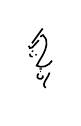
\begin{tikzpicture}[x=.04cm,y=.04cm,baseline=0pt]\draw[line width=.6pt] (1.2,17.3)--(4.6,22.0);\draw[line width=.6pt] (.2,16.5)..controls(.1,15.6)and(.8,15.6)..(1.3,16.0)--(3.4,18.3);\draw[line width=.6pt] (3.8,19.4)--(4.7,19.9)..controls(5.6,19.3)and(5.8,18.4)..(5.8,17.0)..controls(5.5,14.2)and(3.6,12.2)..(2.7,10.2)..controls(4.2,9.3)and(6.5,10.0)..(7.6,11.8);\draw[line width=.55pt,line cap=round] (1.3,14.7)--(1.5,14.9);\draw[line width=.55pt] (.5,14.0)..controls(.3,13.3)and(.8,13.1)..(1.4,13.0);\draw[line width=.5pt] (2.3,13.5)--(2.7,13.8);\draw[line width=.5pt] (3.6,9.1)--(4.3,9.2);\draw[line width=.6pt] (3.3,7.7)..controls(2.5,6.7)and(2.9,5.9)..(4.1,6.0)..controls(4.8,6.1)and(4.7,6.7)..(4.6,7.1);\draw[line width=.6pt] (6.8,8.0)..controls(6.4,6.6)and(5.1,5.3)..(5.0,4.3)..controls(4.9,3.8)and(5.2,3.4)..(5.6,3.2);\draw[line width=.35pt] (3.8,8.2)--(4.0,8.5);\end{tikzpicture}}\figure{\begin{tikzpicture}[x=.03cm,y=.03cm,baseline=0pt]\draw[line width=.6pt] (.7,34.5)--(.8,34.1);\draw[line width=.45pt] (.8,33.3)--(.8,32.9);\draw[line width=.35pt] (.7,32.4)--(.7,32.1);\draw[line width=.45pt] (.6,31.6)--(.3,30.7);\draw[line width=.6pt] (.2,24.9)--(.2,24.2);\draw[line width=.6pt] (.2,23.8)..controls(.2,21.2)and(.1,19.1)..(.3,17.8);\draw[line width=.6pt] (.2,16.3)--(.2,15.5);\draw[line width=.45pt] (.2,15.1)--(.2,14.6);\draw[line width=.45pt] (.2,14.2)--(.2,13.8);\draw[line width=.55pt,line cap=round] (.2,13.0)--(.2,12.8);\draw[line width=.6pt] (-.1,9.0)..controls(.0,6.7)and(.5,4.2)..(.5,1.8);\draw[line width=.65pt,line cap=round] (.4,.9)--(.5,.8);\end{tikzpicture}}}\handwritten{semi-simplicial sont aussi les $\pi_i$ au sens Gr-n-catégories,}
\handwritten{savoir les objets à isom près dans divers \uline{Hom}$(1,1)$\,..... . \deleted{Il y a
aussi une interprétation de l'opération $\Omega$ : \unsure{esp} des lacets
en termes d'opération du shift géométrique évidente sur les
n-catégories.....}}

\margin{11}

\scanpage{13}
\mspage{\handwritten{11}}

III Point de vue ``motivique'' en théorie du cobordisme.

Soit C la catégorie des variétés différe\unsure{\deleted{b}n|\deleted{n}b|b}tiables\inserted{\begin{tabular}[b]{@{}l@{}}\handwritten{(compactes?)}\\[-.6ex]\begin{tikzpicture}[x=1cm,y=1cm,baseline] \draw (0,-.5) .. controls (-.01,-.2) and (.02,-.12) .. (.18,-.02) .. controls (.6,.18) and (1.5,.12) .. (1.8,.17) .. controls (2.1,.19) and (2.25,.28) .. (2.23,.4); \end{tikzpicture}\end{tabular}} (pas nécessairem\unsure{e}\\
ori\unsure{e|n|a}\unsure{n|h|b}tables), \inserted{\begin{tabular}[b]{@{}l@{}}les morphismes étant les classes d'homotopie d'applications continues\\[-.6ex]\begin{tikzpicture}[x=1cm,y=1cm,line width=.4pt]\draw (.10,.40)..controls(-.18,.20)and(-.12,.02)..(.18,0)--(.67,-.02);\draw (.72,-.02)--(.77,-.02);\draw (.88,-.03)--(.94,-.03);\draw (1.08,-.03)--(1.13,-.03);\draw (1.28,-.02)--(1.46,-.02);\draw (1.68,-.02)--(1.75,-.02);\draw (1.96,-.03)--(2.02,-.03);\draw (2.18,-.04)..controls(2.43,-.07)and(2.67,-.08)..(2.78,-.19)..controls(2.83,-.29)and(2.84,-.50)..(2.81,-.53)..controls(2.66,-.23)and(2.85,-.08)..(2.95,-.05);\draw (3.02,-.04)--(3.11,-.03);\draw (3.19,-.03)--(3.29,-.03);\draw (3.39,-.03)--(3.57,-.02);\draw (3.78,-.02)--(3.88,-.03);\draw (3.97,-.03)--(4.15,-.04);\draw (4.27,-.04)--(4.31,-.04);\draw (4.40,-.04)--(4.44,-.04);\draw (4.51,-.04)--(4.94,-.02);\draw (5.06,-.02)--(5.19,-.02);\draw (5.31,-.02)--(5.50,-.02);\draw (5.62,-.02)--(5.66,-.02);\draw (5.77,-.01)--(6.05,-.01);\draw (6.23,-.01)--(6.30,-.01);\draw (6.42,-.01)--(6.47,-.01);\draw (6.59,-.01)--(6.65,-.01);\draw (6.82,-.01)--(6.89,-.01);\draw (7.04,-.01)--(7.15,-.02);\draw (7.33,-.02)--(7.44,-.02);\draw (7.55,-.02)--(7.62,-.02);\draw (7.72,-.02)--(7.80,-.02);\draw (7.98,-.03)--(8.12,-.03);\draw (8.35,-.04)--(8.47,-.04);\draw (8.60,-.04)--(8.67,-.05);\draw (8.81,-.05)--(9.05,-.06);\draw (9.17,-.06)--(9.29,-.07);\end{tikzpicture}\end{tabular}} Si B est une catégorie, on s'intéresse aux couples\\
$(F.,F^{\cdot})$ d'un foncteur covariant et d'un foncteur contravariant de C\\
dans B, satisfaisant les conditions que pour tout $X\in \mathrm{Ob}\, C$, on a $F.(X)=$\\
$F^{\cdot}(X)$, et que si on a un produit fibré ordinaire
\diagram{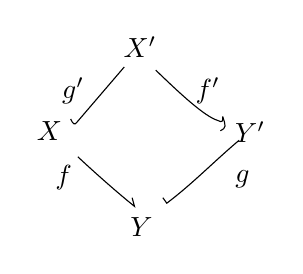
\begin{tikzpicture}[x=1cm,y=1cm,baseline] \node at (1.05,2.2) {$X'$}; \node at (-.1,1.14) {$X$}; \node at (2.45,1.12) {$Y'$}; \node at (1.07,-.08) {$Y$}; \node at (.2,1.65) {$g'$}; \node at (1.91,1.65) {$f'$}; \node at (.08,.55) {$f$}; \node at (2.35,.52) {$g$}; \draw (.85,1.95) -- (.25,1.25) .. controls (.22,1.21) and (.2,1.22) .. (.17,1.29); \draw (1.25,1.91) .. controls (1.55,1.62) and (1.87,1.32) .. (2.04,1.27) .. controls (2.09,1.24) and (2.11,1.26) .. (2.1,1.32); \draw (2.1,1.32) .. controls (2.14,1.2) and (2.15,1.18) .. (2.07,1.14); \draw (.26,.81) .. controls (.56,.53) and (.83,.3) .. (.98,.18) -- (.95,.29); \draw (2.31,1.02) .. controls (2,.76) and (1.71,.46) .. (1.39,.22) -- (1.34,.29); \end{tikzpicture}},
avec f et g transversaux, alors on a $g^{\cdot}f. = f!\,g'^{\cdot}$\inserted{\begin{tabular}[b]{@{}l@{}}(on pose $f.=F.(f)$,$f^{\cdot}=F^{\cdot}\unsure{(}$\\[-.6ex]\begin{tikzpicture}[x=1cm,y=1cm,baseline] \draw (.05,1) .. controls (-.2,.48) and (.05,.22) .. (.65,.16) -- (.95,.14) .. controls (1.1,.11) and (1.03,-.2) .. (1.08,-.62) .. controls (1.1,-.16) and (1.03,-.05) .. (1.25,.11) .. controls (2.2,.32) and (3.4,.42) .. (4.65,.24); \end{tikzpicture}\end{tabular}}. La question est\\
de trouver une B et un couple $(F.,F^{\cdot})$ qui soient ``universels'' dans \unsure{u\unsure{n}|w|u}\\
sens évident. Quillen prouve que la construction suivante donne une\\
telle solution.

Pour toute variété $X\in \mathrm{ob}\, C$ , on définit un anneau commutatif\\
B(X) (l'anneau de bordisme de X) en prenant comme éléments les class\unsure{e}\\
\deleted{de} d'éléments de C au dessus de X, pour la relation de cobordisme:\\
$f'{:}X'\rightharpoonup X$ et $f''{:}X''\rightharpoonup X$ sont équivalents, s'il existe une variété à bord\\
Z, et un $f{:}Z\to X$, tel que bord $Z = X'\handwritten{\amalg} X''$ et $f'$ et $f''$ sont induits\\
par f. La somme de B(X) est la somme disjointe (c'est une loi de grou\unsure{p}\\
\deleted{l'i\unsure{n}verse étant} où tout élément est d'ordre \deleted{1}\handwritten{2} \deleted{\unsure{ou} 2}), le produit est\\
donné par le produit fibré, en utilisant le théorème de tra\unsure{n|h|b}sversalit\unsure{e}\\
de Thom pour bouger un peu f'', de sorte à le rendre transversal à f'.
\margin{\handwritten{\uline{NB} L'anneau est de plus \uline{gradué} par la dimension relative ....}}

Si on a $f{:}\ X\rightharpoonup Y$, on définit $f. : B(X)\to B(Y)$ de façon évidente (tou\unsure{t}\\
variété sur X est sur Y), et $f^{\cdot}{:}\ B(Y)\to B(X)$ par produit fibré (uti\unsure{l}\\
sant encore le th. de transversalité). De cette façon, B(X) devient u\unsure{n|r}\\
foncteur-anneau \inserted{\begin{tabular}[b]{@{}l@{}}\handwritten{(g\unsure{ra}du\unsure{é|e})}\\[-.6ex]\begin{tikzpicture}[x=1cm,y=1cm,baseline] \draw (.12,-.9) .. controls (-.18,-.95) and (-.12,.02) .. (.2,.22) .. controls (.45,.45) and (1.1,.6) .. (1.55,.65); \draw (1.65,.65) .. controls (1.95,.73) and (2.65,.7) .. (2.85,.73) .. controls (3.15,.76) and (3.65,.97) .. (3.63,1.26); \end{tikzpicture}\end{tabular}} contravariant en X, et un foncteur groupe covariant e\unsure{n|r}

\margin{\handwritten{12}}

\scanpage{14}
\mspage{12}

X. De plus, on a la formule\rlap{\raisebox{-.1ex}{\begin{tikzpicture}[x=.45cm,y=.45cm,baseline=0pt]\draw[line width=.4pt] (1,2.34)--(.93,2.31);\draw[line width=.4pt] (.81,2.25)--(.78,2.23);\draw[line width=.4pt] (.53,2)--(.5,1.98);\draw[line width=.4pt] (.43,1.89)--(.39,1.82);\draw[line width=.4pt] (.33,1.72) .. controls (.16,1.42) and (.27,1.23) .. (.59,1.09) .. controls (.81,.98) and (.98,1.05) .. (1.23,.99) .. controls (1.4,.94) and (1.58,.94) .. (1.71,.94) .. controls (1.87,.94) and (1.81,.72) .. (1.65,.6);\draw[line width=.4pt] (1.94,.73) .. controls (2.02,.79) and (2.09,.81) .. (2.2,.81);\draw[line width=.4pt] (2.79,.83)--(2.83,.83);\draw[line width=.4pt] (2.89,.83)--(3.33,.81);\draw[line width=.4pt] (3.4,.81)--(3.54,.82);\draw[line width=.4pt] (1.8,.32)--(1.9,.04);\end{tikzpicture}}}\inserted{\handwritten{du type $g^{\bullet}f_{\bullet}=f'_{\bullet}g'^{\bullet}$ ci-dessus, impliquant la \uline{formule}\rlap{\hspace{-0.8em}\raisebox{1.6ex}{\begin{tikzpicture}[x=.2cm,y=.2cm,baseline=0pt]\draw[line width=.4pt] (0,0) .. controls (.2,.02) and (.4,-.02) .. (.55,-.02);\draw[line width=.4pt] (.63,-.02) .. controls (.9,-.03) and (1.15,-.1) .. (1.4,-.16);\end{tikzpicture}}}}} de projection habituelle. Ceci posé, les
constructions bien connues en théorie des correspondances permettent
de définir une catégorie $\underline{B}$ dont lds objets sont ceux de C, et les
Hom étant donnés par
\[
\mathrm{Hom}_{B}(X,Y)=B(XxY)\quad .
\]
On a un isomorphisme canonique $\underline{B}\simeq\underline{B}^{o}$ , qui est l'identité sur les
objets et la symmétrie $B(XxY)\simeq B(YxX)$ sur les flêches, et un foncteur
évident \deleted{$\unsure{C}\,\unsure{:}\,\underline{B}$} $F.$ : $C\rightharpoonup\underline{B}$ , qui est l'identité sur les objets et don\unsure{n}
par les graphes sur les flêches. Composé avec la symmétrie précédente
on trouve un foncteur $F^{\bullet}$: \deleted{$\unsure{B}($} $C\rightharpoondown\underline{B}$. On vérifie enfin que le couple
($F.$,$F^{\bullet}$) satisfait aux conditions envisagées dans l'alinéa 1 (ceci aus\illegible{1}
devrait être formalisé au cas des correspondances géné rales ...). \unsure{\deleted{D}O|\deleted{L}O|\deleted{O}D|\deleted{O}L}\unsure{\deleted{a}n|\deleted{n}a}
vérifie enfin qu'il a la propriété universelle qu'il faut. Lorsqu'on
se donne un couple ($F!$,$F'^{\bullet}$) à val eursdans une catégorie B', il faut
trouver une factorisation par B. Elle est toute trouvée sur les
objets, il faut la définir sur les flêches, donc définir, pour X,Y
dans C, une application
\[
(*)\qquad B(XxY)\to\mathrm{Hom}(X',Y')\quad .
\]
Mais si Z est au\unsure{\deleted{d}-|\deleted{-}d|\deleted{a}d|\deleted{d}a}dessus de XxY, d'où $p:Z\rightharpoonup X$ et $q:Z\rightharpoondown Y$, on lui assoc
un élément du deuxième membre de (*) comme le composé
\[
X'\xrightarrow{F'^{\bullet}(p)}Z'\xrightarrow{F!(\unsure{q})}Y'\quad .
\]
Il faut prouver que l'élément obtenu en remp\unsure{\deleted{l}a|\deleted{a}l}çant Z\inserted{\begin{tabular}[b]{@{}l@{}}\handwritten{$\unsure{(=}\unsure{Z}_{\unsure{o}})$}\\[-.9ex]
\begin{tikzpicture}[x=.45cm,y=.45cm,baseline=0pt]\draw[line width=.4pt] (.28,1.83)--(.37,1.8);\draw[line width=.4pt,line cap=round] (.15,1.67)--(.16,1.67);\draw[line width=.4pt] (.12,.57)--(.06,.48);\draw[line width=.4pt,line cap=round] (.03,.38)--(.04,.38);\draw[line width=.4pt] (.02,.16)--(.05,.08);\end{tikzpicture}
\end{tabular}} par un $Z_1$ cobor\unsure{\deleted{a}d|\deleted{d}a}
dant au dessus de X\inserted{\begin{tabular}[b]{@{}l@{}}\handwritten{\unsure{e}st le \unsure{même}}\\[-.9ex]
\begin{tikzpicture}[x=.7cm,y=.7cm,baseline=0pt]\draw[line width=.4pt] (0,0) .. controls (.24,.18) and (.48,.3) .. (.7,.31) .. controls (1.15,.31) and (1.9,.22) .. (2.28,.29);\draw[line width=.4pt,line cap=round] (2.57,.34)--(2.59,.34);\draw[line width=.4pt] (2.65,.35)--(3.02,.4);\draw[line width=.4pt] (3.12,.43)--(3.85,.56)--(3.77,.67);\draw[line width=.4pt,line cap=round] (4.08,.55)--(4.1,.55);\end{tikzpicture}
\end{tabular}}. Or si $g$: $T\rightharpoonup XxY$ réalise le cobordisme, on
voit (regardant seulement T et la décomposition bord(T) = $Z_{\handwritten{\unsure{o|0}}}\amalg Z_1$)
qu'il existe une variété $\overline{T}$ sur $S^1$ (obtenue en ``doublant'' T) \deleted{et une}
\deleted{application T \unsure{une}} tr\unsure{\deleted{q}a|\deleted{a}q}nsversale au dessus d'un couple de poihts $s_o$,s
de $S^1$, tels que $Z_i$ soit l'image inverse \inserted{\begin{tabular}[b]{@{}l@{}}\handwritten{dans $\overline{T}$}\\[-.9ex]
\begin{tikzpicture}[x=.68cm,y=.68cm,baseline=0pt]\draw[line width=.4pt] (3.25,1.65) .. controls (3.34,1.4) and (3.26,1.27) .. (3.12,1.25) .. controls (2.5,1.18) and (1.45,1.14) .. (.73,1.06) .. controls (.4,1.05) and (.12,.91) .. (.05,.63) .. controls (-.02,.36) and (.07,.17) .. (.25,0);\end{tikzpicture}
\end{tabular}} de $s_i$ (i=0,1); d'autre part,

\margin{13}

\scanpage{15}
\mspage{13}

g manifestement se prolonge en $\overline{g}$ : $\overline{T}\rightharpoondown XxY$ . Cela nous ramène à prouv
que \inserted{le composé} \handwritten{(}$\handwritten{\unsure{t|\dagger}\,\unsure{i}}\overline{T}'\xrightarrow{\handwritten{\alpha_i}}\handwritten{\unsure{t|\dagger|F}}Z'_i\overset{\handwritten{\alpha_{i\unsure{*}}}}{\rightharpoondown}\handwritten{\unsure{t|\dagger}}\overline{T}'$ ne dépend pas de i=0,1. Ecrivons X au lieu de $\overline{T}'$, \unsure{'}

considérons le diagramme cartésien d'inclusions
\diagram{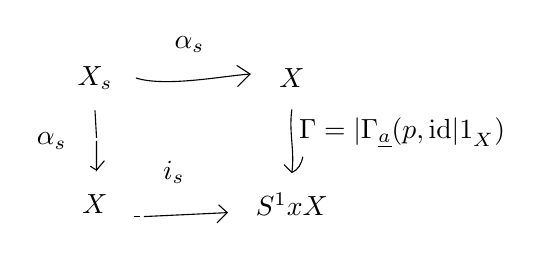
\begin{tikzpicture}[x=1cm,y=1cm,baseline] \node at (0,1.6) {$X_s$}; \node at (2.5,1.6) {$X$}; \node at (0,0) {$X$}; \node at (2.5,0) {$S^1xX$}; \node at (1.2,2.02) {$\alpha_s$}; \node at (-.55,.8) {$\alpha_s$}; \node at (1,.4) {$i_s$}; \node at (3.9,.9) {$\unsure{\Gamma=|\Gamma_{\underline{a}}}\unsure{(}p,\unsure{\mathrm{id}|1}_X)$}; \draw (.52,1.6) .. controls (.9,1.48) and (1.65,1.63) .. (1.97,1.65); \draw (1.8,1.76) -- (1.97,1.65) -- (1.81,1.49); \draw (0,1.19) -- (.02,.84); \draw (.02,.8) -- (.02,.43) -- (.12,.55); \draw (.02,.43) -- (-.06,.48); \draw (2.5,1.2) .. controls (2.46,.9) and (2.54,.68) .. (2.5,.4); \draw (2.4,.5) -- (2.5,.4) .. controls (2.57,.42) and (2.63,.52) .. (2.64,.6); \draw (.49,-.16) -- (.57,-.16); \draw (.62,-.16) -- (1.68,-.11); \draw (1.57,-.01) -- (1.68,-.11) -- (1.55,-.24); \end{tikzpicture}},

on a alors $\handwritten{\alpha}^{\handwritten{*}}_s\,\handwritten{\unsure{\alpha}}_{s*}=\handwritten{\Gamma}^{\handwritten{*}}i_{s\handwritten{\unsure{*}}}$ , qui ne dépend pas de s puisque $i_s$ n'en
dépend pas à homotopie près. - Le reste est sans doute l'AQT.

Sur la strcture des B.(X). Ce sont tous des algèbres graduées
sur B.(pt)=\handwritten{$\Lambda$} , qui est une algèbre graduée à degrés positifs, réduit
\margin{\figure{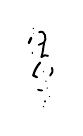
\begin{tikzpicture}[x=.5em,y=.5em,line cap=round,line join=round]
\fill (.38,6.15) circle (.055);
\fill (.40,5.78) circle (.03);
\draw[line width=.7pt] (.80,5.88) .. controls (1.23,6.08) and (1.37,5.37) .. (1.15,5.11) .. controls (1.10,4.75) and (1.05,4.31) .. (.96,4.08) .. controls (1.12,4.25) and (1.29,4.23) .. (1.44,4.17);
\draw[line width=.65pt] (1.18,5.14) -- (.76,4.96);
\draw[line width=.9pt] (.22,5.46) -- (.06,5.10);
\fill (.31,4.38) ellipse (.055 and .09);
\draw[line width=.8pt] (.87,3.68) .. controls (.61,3.40) and (.45,3.04) .. (.37,2.75) .. controls (.45,2.65) and (.53,2.64) .. (.64,2.63);
\fill (1.12,3.02) circle (.045);
\draw[line width=.7pt] (1.72,3.30) .. controls (1.84,3.04) and (1.71,2.88) .. (1.59,2.74);
\fill (1.29,2.34) circle (.05);
\fill (1.38,1.84) circle (.05);
\draw[line width=.65pt] (.72,1.72) .. controls (.83,1.67) and (.94,1.67) .. (1.02,1.67);
\fill (1.55,1.23) circle (.04);
\fill (1.22,.88) ellipse (.07 and .10);
\fill (1.11,.50) circle (.055);
\end{tikzpicture}}}
à $\underline{F}_2$ en degré\deleted{\unsure{z|s}} 0. C'est d'ailleurs une algèbre de polynômes \inserted{\begin{tabular}[b]{@{}l@{}}\handwritten{à une infinité de générateurs $X_i$ ($i$ entier \unsure{$\geq|>$} \illegible{2}}\\[-.6ex]\begin{tikzpicture}[x=.6cm,y=.6cm,baseline] \draw (.12,.45) .. controls (-.2,.13) and (-.13,-.06) .. (.12,-.15) .. controls (.32,-.21) and (.5,-.2) .. (.76,-.29); \end{tikzpicture}\end{tabular}} connue\,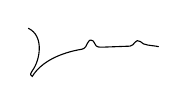
\begin{tikzpicture}[x=.65cm,y=.65cm,baseline] \draw (0,.45) .. controls (.32,.3) and (.23,-.18) .. (.08,-.38) .. controls (.05,-.44) and (.02,-.45) .. (.08,-.49) .. controls (.25,-.21) and (.62,-.03) .. (1.05,.04) .. controls (1.19,.07) and (1.13,.28) .. (1.27,.2) .. controls (1.34,.1) and (1.3,.08) .. (1.45,.08) -- (1.99,.1) .. controls (2.08,.11) and (2.09,.26) .. (2.19,.19) .. controls (2.25,.11) and (2.4,.12) .. (2.55,.09); \end{tikzpicture}
On a un homomorphisme évident \inserted{d'anne\unsure{\deleted{d}a|\deleted{a}d}\unsure{\deleted{t}u|\deleted{u}t}xp\unsure{\deleted{d}g|\deleted{g}d|g}\unsure{\deleted{i}r|\deleted{r}i}adués} B.(X) $\to H^{\handwritten{\unsure{B}}}(X)$, nul en degrés \handwritten{$>$}0, qui
\margin{\handwritten{\uline{NB} $H^*(X)$ $(=H^*(X,\mathbb{F}_2)$}}
à tout Z sur X associe l'image de 1 \handwritten{$\in$} $H^o(Z)$ par l'homomorphisme de Gys
\margin{\handwritten{en fait $H(X)\simeq B.(X)/\Lambda^+B.(X)$}}
associé à Z$\to$ X. Cet homomorphisme par Thom est surjectif (toute cla
se de cohomologie provient d'une image de variété compacte....); \deleted{\unsure{n}ote}

On ppouve même qu'il existe un relèvement fonctoriel en X
\margin{\handwritten{?}}
$H^\bullet$(X) $\to$ B.(X), \inserted{\begin{tabular}[b]{@{}l@{}}\handwritten{il est douteux qu'il soit}\\[-.6ex]\begin{tikzpicture}[x=1.35cm,y=.6cm,line width=.4pt]\draw (.11,.67)..controls(-.15,.24)and(-.13,-.37)..(.05,-.47);\draw (.21,-.25)..controls(.30,-.18)and(.42,-.14)..(.58,-.14);\draw (.62,-.14)--(.72,-.14);\draw (.78,-.14)--(.82,-.14);\draw (.89,-.14)--(.94,-.14);\draw (1.00,-.14)--(1.02,-.14);\draw (1.12,-.14)--(1.13,-.14);\draw (1.17,-.14)--(1.18,-.14);\draw (2.61,-.16)--(2.64,-.16);\draw (2.71,-.16)--(2.73,-.16);\draw (2.80,-.16)--(2.82,-.16);\draw (3.49,-.14)--(3.51,-.14);\draw (3.58,-.14)--(3.65,-.14);\draw (3.74,-.14)--(3.84,-.13);\draw (3.92,-.13)--(3.96,-.13);\draw (4.04,-.12)--(4.06,-.12);\draw (4.3,.64)..controls(4.35,.24)and(4.36,.12)..(4.08,.03);\end{tikzpicture}\end{tabular}} compatible avec multiplication\handwritten{)} \deleted{t\unsure{e}l}tel que l'on ait:

\deleted{a)} L'homomorphisme correspondant $H^\bullet(X)\otimes_{\underline{F}_2}\handwritten{\Lambda}\simeq$ B.(X) est un iso
\margin{\handwritten{?}}
morphisme (ce sera vrai pour tout relèvement individuellement ...), e

\deleted{b)}\handwritten{[}\deleted{Le}\inserted{\begin{tabular}[b]{@{}l@{}}\handwritten{Quillen ignore si}\\[-.6ex]\begin{tikzpicture}[x=1cm,y=.6cm,line width=.4pt]\draw (.08,-.25)..controls(.01,-.12)and(-.03,.04)..(-.03,.14);\draw (-.03,.25)--(-.03,.33);\draw (-.02,.42)--(.01,.53);\draw (.04,.59)--(.10,.66);\draw (.15,.70)--(.34,.76);\draw (.40,.78)--(.44,.79);\draw (2.35,.75)--(2.43,.75);\draw (2.50,.75)--(2.58,.74);\draw (2.64,.74)--(2.82,.73);\draw (2.89,.73)--(2.96,.73);\draw (3.05,.72)--(3.26,.71);\draw (3.40,.70)--(3.68,.69);\draw (3.77,.69)--(3.98,.68);\draw (4.08,.68)..controls(4.56,.71)and(4.65,.85)..(4.65,1.02);\end{tikzpicture}\end{tabular}} relèvement est compatible aussi avec les hom. de Gysin

Ainsi, la catégorie $\underline{B}$ admet un foncteur pleinement fidèle dans la
catégorie des modules gradués libres de type fini sur \handwritten{$\Lambda$}, les modules
de type fini qu'on obtient ainsi ayant des générateurs à degrés \handwritten{$<$} 0
satisfaisant (pour X connexe i.e. quand il y a un seul générateur de
\margin{\handwritten{ie. l'enveloppe ``Karoubienne''}}
degré zéro\handwritten{)}\rlap{\hspace{-.4em}\raisebox{-.4ex}{\begin{tikzpicture}[x=.6cm,y=.6cm,line width=.4pt]\draw (.7,-.05)..controls(.45,-.24)and(.13,-.11)..(.01,-.08)..controls(-.05,-.06)and(-.1,-.13)..(-.12,-.17);\draw (-.17,-.25)--(-.23,-.35);\draw (.57,-.15)..controls(.78,-.11)and(.92,-.03)..(.98,.08);\end{tikzpicture}}} la dualité de Poincaré. Quand on prend la catégorie \uline{quas}
\uline{abélienne}\inserted{\handwritten{B}}-associée à $\underline{B}$, on trouve donc tous les modules gradués libre
de type fini à générateurs \deleted{négatifs} en degrés \handwritten{$\leqslant$} 0 seulement. C'est u\illegible{1}

\margin{14}

\scanpage{16}
\mspage{\handwritten{14}}
\margin{\handwritten{$=$ karoubie\unsure{nne|n} $+$ additive}}

catégorie \inserted{\begin{tabular}[b]{@{}l@{}}additive(\unsure{et|ct} même quasi-abélienne)\\[-.6ex]\begin{tikzpicture}[x=1cm,y=.6cm,line width=.35pt]\draw (5.5,.8)..controls(5.52,1.02)and(5.56,1.05)..(5.8,1.05)..controls(6.8,1.05)and(7.3,.85)..(8.9,.94)..controls(9.2,.96)and(9.25,.96)..(9.3,.76);\draw (.12,-.35)..controls(-.06,-.05)and(-.02,.16)..(.25,.18)..controls(.7,.3)and(1,.26)..(1.45,.24);\draw (3.95,.21)--(4.5,.2)--(5.25,.2)--(5.95,.2);\draw (6.05,.2)..controls(7.5,.12)and(8.7,.22)..(10.1,.27)..controls(11.1,.3)and(11.7,.54)..(11.66,1.05);\end{tikzpicture}\end{tabular}} avec $\unsure{\otimes|0}$ qui a toutes les vertus, sauf d'être abélienne, et
sauf d''admettre des \uline{Hom} internes. Pour trouver ces derniers, on peu
si on veut paraphraser la construction de la catégorie des motifs,
\deleted{introduisant un motif} \inserted{\handwritten{en}} considérant l'objet \inserted{\begin{tabular}[b]{@{}l@{}}\handwritten{$\Lambda^{\unsure{\prime}}(-1)$}\\[-.6ex]\begin{tikzpicture}[x=.1mm,y=-.1mm,line cap=round,line join=round]\draw[line width=.45pt] (74,78) .. controls (73,58) and (89,47) .. (115,44);\draw[line width=.35pt] (119,42) -- (125,40);\draw[line width=.45pt] (126,39) .. controls (141,27) and (147,13) .. (146,10);\end{tikzpicture}\end{tabular}} de $\overset{\handwritten{\sim}}{\underline{B}}$ conoyau de
$p^{\handwritten{*}} : e \rightharpoonup S$, où $p:S^1 \rightharpoonup e$ est l'application du cercle sur un
point. C'est un objet de poids 1 (le poids est défini par le degré
des générateurs, changés de signe). On constate aussitôt que le
foncteur $M \unsure{\mapsto} M(-1) = M\otimes \handwritten{\Lambda}(-1)$ de $\overset{\handwritten{\sim}}{\underline{B}}$ dans lui-même est pleinement fidèl
ce qui permet alors, par une construction formelle standard, de com
\inserted{\begin{tabular}[b]{@{}l@{}}\handwritten{\unsure{lé|plé}}\\[-.6ex]\begin{tikzpicture}[x=.1mm,y=-.1mm,line cap=round,line join=round]\draw[line width=.5pt] (59,11) .. controls (62,20) and (46,31) .. (29,38) .. controls (26,49) and (27,57) .. (27,62);\end{tikzpicture}\end{tabular}}ter $\overset{\handwritten{\sim}}{\underline{B}}$ en une catégorie où $\handwritten{\Lambda}(-1)$ devient inversible. Il se trouve
alors que dans cette dernière les \uline{Hom}(X,Y) internes existent et
\deleted{s\unsure{a}tisf\unsure{o}\unsure{n}t} sont isomorphes à $\overset{\handwritten{\vee}}{X}\otimes Y$, ... en fait , on trouve maintenant\handwritten{\unsure{l|(}}
catégorie de\deleted{s} \uline{tous} les modules gradués libres de type fini sur $\handwritten{\Lambda}$.
Bien sûr, cette catégorie n'est pas encore abélienne pour autant,
puisque $\handwritten{\Lambda}$ n'est pas un corps; \deleted{pour} \inserted{si on veut} définir la catégorie abélienne
engendrée, on s'attend à trouver l\unsure{a|\deleted{e}a|\deleted{a}e}\deleted{s} catégorie desmodules de \deleted{type} \inserted{\handwritten{présentati-}} f
\margin{\figure{\begin{tikzpicture}[x=.3mm,y=.3mm,line cap=round,line join=round]\draw[line width=.65pt] (0,25) .. controls (2,27) and (4,29) .. (6,27) .. controls (8,25) and (8,23) .. (8,21) .. controls (9,20) and (9,18) .. (8,17) .. controls (5,15) and (3,12) .. (2,11) .. controls (4,10) and (7,13) .. (9,13) .. controls (9,11) and (6,8) .. (5,7) -- (5,5) .. controls (7,7) and (9,7) .. (10,6) -- (10,3) .. controls (9,1) and (8,0) .. (7,-2) -- (9,-2);\draw[line width=.7pt] (1.4,22.1) -- (1,21.7);\draw[line width=.7pt] (.6,18.3) -- (1.4,18.1);\end{tikzpicture}}}sur $\handwritten{\Lambda}$.( \inserted{\handwritten{qui est \unsure{cohérent|abélienne|abélien} bien que $\Lambda$ ne soit pas \unsure{noethérien|noéthérien}, car $\Lambda$ est}} \deleted{est-il noethérien, j.e. le nombre de générateurs est-il
fini ? )}\handwritten{ $\underset{\unsure{\rightharpoondown|\longrightarrow}}{\lim}$ d'anneaux noeth\unsure{.|,} à hom de transition \uline{plats} )}.

Cette construction ressemblerait à celle d'une théorie des
motifs où on n'aurait pas passé à l'équivalence homologique pour
les cycles, mais où on aurait gardé l'équivalence rationelle, - qui
est bien trop fine \deleted{p\unsure{ou|eu}}à beaucoup d'égards. Pour trouver un équiva
lent plus étroit, il convin\unsure{\deleted{t}n|\deleted{n}t}t de reprendre la théorie prédédente,on
pourrait formuler le même Pb universel que plus haut, mais en prena
l'équivalence homologique (via le graphe) des morphismes de variété
au lieu de l'équivalence homotopique. \deleted{Mais alors il semble que l'on
trouve comme catégorie solution celle dont les objets sont les vari}

\margin{\handwritten{15}}

\scanpage{17}
\mspage{15}

\deleted{tés, les morphismes \uline{toutes} les correspondances \inserted{co}homologiques (\unsure{e|o}n ve
du thorème de Thom rappelé plus haut). On trouve donc un foncteur
pleinement fidèle de cette catégorie dans \unsure{c|o}elle des vectoriels
gradués d\deleted{\unsure{e}} d positivement de dim. finie sur $\underline{F}_2$ , qui est déjà abéli
ne, et si on veut rendre comme plus haut $\underline{F}_2(-1)$ inversible, on trou
tous les vectoriels gradués de dim. finie sur $\underline{F}_2$. C'est un peu tr\unsure{o}
trivial comme structure, et on peut faire mieux,} \deleted{\unsure{e|E}n prenant comme}
\inserted{Pour trouver une catégorie universelle,}
\deleted{correspondances Pour c\unsure{e}ci} on associe à toute X
\deleted{l\unsure{e|a} \unsure{sous} \unsure{anneau} ensem\unsure{b}}
\deleted{\unsure{d|l}} l'ensemble \inserted{\begin{tabular}[b]{@{}l@{}}S(X)\\[-.6ex]\begin{tikzpicture}[x=1cm,y=1cm,baseline=0pt]\draw[line width=.4pt] (0,0)--(.03,.05);\draw[line width=.4pt] (.08,.13)--(.15,.2);\draw[line width=.4pt] (.22,.28)--(.43,.51);\draw[line width=.4pt] (.49,.58)--(.63,.75);\draw[line width=.4pt] (.67,.8)--(.69,.83);\end{tikzpicture}\end{tabular}} des sous-variétés \deleted{S(X)} de X, modulo équivalence hom\unsure{o}
gique. Donc S(X) $\subset$ H$^{\bullet}$(X), et on prouve qu'on trouve en fait un sous
anneau de H$^{\bullet}$(X) (grâce à un théorème de Thom qui caractérise S(X) \handwritten{e\unsure{n|t}}
termes d'opérations de Steenrod, cf plus bas). On prouve de même
(par le même théorème) que les S(XxY) sont stables par composition
correspondances cohomologiques( cela ne semble pas trivial, puisque
les S(X) ne sont pas stables par Gysin...). D'où une catégorie ad\unsure{d|c}
tive dont les objets sont ceux de C, les flêches sont les \inserted{\begin{tabular}[b]{@{}l@{}}\handwritten{él. des}\\[-.6ex]\begin{tikzpicture}[x=1cm,y=1cm,baseline=0pt]\draw[line width=.4pt] (0,.5) .. controls (.22,.28) and (.67,.32) .. (.99,.33) .. controls (1.16,.4) and (1.3,.44) .. (1.44,.37) .. controls (1.48,.32) and (1.47,.14) .. (1.53,.13) .. controls (1.66,.35) and (1.88,.49) .. (2.13,.48) .. controls (2.38,.42) and (2.61,.4) .. (2.77,.55) .. controls (2.86,.66) and (2.91,.76) .. (2.9,.84)--(2.78,.85);\draw[line width=.4pt] (1.53,.13)--(1.5,-.15);\end{tikzpicture}\end{tabular}} S(XxY),
Il semble qu'elle doive jouer le rôle universel que j'ai envisagé
plus haut. En tous cas, sa définition géo\unsure{\deleted{é}m|\deleted{m}é}\unsure{\deleted{m}é|\deleted{é}m}trique est fort simple
Nous allons en donner une interpétation algébrique. P\unsure{\u{o}}ur ce\unsure{\deleted{i}c|\deleted{c}i}\unsure{\deleted{c}i|\deleted{i}c},
considérons l'anneau des opérations cohomologiques \inserted{``stables''} \deleted{additives sur \unsure{l|i}}
\margin{\begin{tikzpicture}[x=1cm,y=1cm,baseline=0pt,line cap=round]\draw[line width=.4pt] (.27,4.8)--(.18,4.57);\draw[line width=.4pt] (.13,4.45)--(.12,4.4);\draw[line width=.4pt] (.08,4.34)--(.08,4.32);\draw[line width=.4pt] (.04,4.25)--(.03,4.2);\draw[line width=.4pt] (-.04,3.96)--(-.04,3.93);\draw[line width=.4pt] (-.05,3.82)--(-.07,3.66);\draw[line width=.4pt] (-.07,3.38)--(-.07,3.29);\draw[line width=.4pt] (-.07,3.2)--(-.07,3.14);\draw[line width=.4pt] (-.06,3.05)--(-.05,2.99);\draw[line width=.4pt] (-.01,2.75)--(0,2.67);\draw[line width=.4pt] (.01,2.57) .. controls (.06,2.36) and (.1,2.11) .. (.14,1.98);\draw[line width=.4pt] (.16,1.85)--(.17,1.65);\draw[line width=.4pt] (.18,1.5)--(.18,1.41);\draw[line width=.4pt] (.17,1.27)--(.17,1.18);\draw[line width=.4pt] (.16,1.02)--(.16,1);\draw[line width=.5pt] (.15,.87)--(.15,.77);\draw[line width=.3pt] (.16,.53)--(.16,.51);\draw[line width=.3pt] (.17,.35)--(.17,.33);\draw[line width=.3pt] (.175,.12)--(.175,.1);\begin{scope}[yshift=-4.2cm]\draw[line width=.25pt] (.05,4.13)--(.05,4.11);\draw[line width=.2pt] (0,3.8)--(0,3.78);\draw[line width=.25pt] (.08,3.15)--(.08,3.13);\draw[line width=.25pt] (.09,2.96)--(.09,2.94);\draw[line width=.4pt] (.11,2.42)--(.11,2.37);\draw[line width=.4pt] (.115,2.31)--(.115,2.25);\draw[line width=.2pt] (.115,2.2)--(.115,2.18);\draw[line width=.2pt] (.12,2.07)--(.12,2.05);\draw[line width=.4pt] (.14,1.68)--(.14,1.63);\draw[line width=.25pt] (.15,1.46)--(.15,1.44);\draw[line width=.4pt] (.14,1.08)--(.14,.92);\draw[line width=.4pt] (.11,.81)--(.1,.7);\draw[line width=.4pt] (.09,.51) .. controls (.09,.39) and (.1,.33) .. (.14,.29);\draw[line width=.2pt] (.19,.15)--(.19,.13);\end{scope}\end{tikzpicture}}
\deleted{des endomorphismes du}
\margin{\figure{\begin{tikzpicture}[x=1cm,y=1cm,baseline=0pt,line cap=round]\draw[line width=.5pt] (1,3.6)--(.91,3.45);\draw[line width=.5pt] (1.35,3.3) .. controls (1.32,3.2) and (1.27,3.08) .. (1.22,3.0);\draw[line width=.5pt] (.8,3.22) .. controls (.65,3.11) and (.43,2.9) .. (.5,2.81) .. controls (.56,2.75) and (.64,2.79) .. (.68,2.85);\draw[line width=.5pt] (.9,3.1) .. controls (1.02,3.2) and (1.1,2.99) .. (1.1,2.83) .. controls (1.1,2.61) and (1.12,2.39) .. (1.06,2.24) .. controls (.94,2.14) and (.77,2.13) .. (.68,2.19)--(.66,2.27);\draw[line width=.5pt] (.99,2.16)--(1.11,2.03)--(1.01,1.97);\draw[line width=.65pt] (.87,2.66)--(.88,2.68);\draw[line width=.5pt] (1,1.92) .. controls (.9,1.75) and (.83,1.6) .. (.77,1.48) .. controls (.67,1.35) and (.57,1.16) .. (.63,1.14);\draw[line width=.5pt] (.75,1.5) .. controls (.91,1.45) and (1.04,1.32) .. (1.13,1.32) .. controls (1.23,1.32) and (1.34,1.36) .. (1.4,1.43);\draw[line width=.5pt] (1.08,1.33)--(1.1,1.15);\draw[line width=.7pt] (1,.55)--(1.02,.58);\end{tikzpicture}}}
\deleted{\deleted{le} foncteur $X\quad H^{\bullet}(X)$ qui sont additifs, et qui en degré zéro se
réduisent à un multiple de l'identité}\begin{tikzpicture}[x=1cm,y=1cm,baseline=0pt]\draw[line width=.4pt] (0,0)--(.18,-.02) .. controls (.23,-.03) and (.25,-.1) .. (.31,-.06) .. controls (.48,.18) and (.63,.51) .. (.78,.83) .. controls (.84,.96) and (.85,1.02) .. (.79,1.08);\end{tikzpicture}
\figure{\begin{tikzpicture}[x=1cm,y=1cm,baseline=0pt]\draw[line width=.4pt] (0,.38) .. controls (.02,.24) and (0,.15) .. (.1,.06)--(.08,0);\draw[line width=.4pt] (.1,.07)--(.36,.33);\draw[line width=.4pt] (.4,.36)--(.45,.39);\draw[line width=.4pt] (.67,.39) .. controls (.71,.2) and (.78,.09) .. (.87,.11) .. controls (1.08,.12) and (1.29,.36) .. (1.45,.35) .. controls (1.56,.32) and (1.56,.14) .. (1.75,.14) .. controls (1.96,.14) and (2.26,.33) .. (2.4,.32) .. controls (2.54,.3) and (2.66,.04) .. (2.82,.04) .. controls (3.14,.04) and (3.48,.11) .. (3.61,.08)--(3.8,.06);\end{tikzpicture}}
C'est un anneau gradué, avec
application diagonale anticommutative \inserted{\begin{tabular}[b]{@{}l@{}}i.e. commutative (car. 2 !)\\[-.9ex]
\begin{tikzpicture}[x=1cm,y=1cm,baseline=0pt]\draw[line width=.4pt] (0,0) .. controls (.13,.12) and (.48,.13) .. (1.16,.13)--(1.18,.12)--(1.18,.075);\draw[line width=.4pt] (1.25,.12)--(1.34,.115);\draw[line width=.4pt] (1.4,.11)--(1.49,.1);\draw[line width=.4pt] (1.58,.09)--(1.7,.08);\draw[line width=.4pt] (1.8,.08)--(1.84,.08);\draw[line width=.4pt] (3.78,.1) .. controls (3.96,.11) and (4.12,.11) .. (4.22,.19);\draw[line width=.4pt] (4.27,.23)--(4.31,.29);\draw[line width=.4pt] (4.38,.33)--(4.4,.38)--(4.33,.38);\end{tikzpicture}
\end{tabular}}, associative et unitaire. So\unsure{n|i}
dual gradué est une algèbre \inserted{\begin{tabular}[b]{@{}l@{}}graduée anti\unsure{o|c}ommutative \begin{tikzpicture}[x=1cm,y=1cm,baseline=0pt]\draw[line width=.35pt](0,-.05)--(.09,-.05);\end{tikzpicture} donc \begin{tikzpicture}[x=1cm,y=1cm,baseline=0pt]\draw[line width=.35pt](0,-.05)--(.09,-.05);\end{tikzpicture}\deleted{commutative};\\[-.9ex]
\begin{tikzpicture}[x=1cm,y=1cm,baseline=0pt,line cap=round]\draw[line width=.5pt] (0,0)--(.01,.01);\draw[line width=.4pt] (.25,.03)--(.26,.03);\draw[line width=.4pt] (.32,.04)--(.64,.06);\draw[line width=.4pt] (.71,.065)--(.78,.07);\draw[line width=.4pt] (.86,.075)--(.96,.09);\draw[line width=.4pt] (1.06,.1)--(1.1,.105);\draw[line width=.4pt] (1.18,.11)--(1.3,.12);\draw[line width=.4pt] (1.42,.13)--(1.53,.14);\draw[line width=.4pt] (1.6,.145)--(1.83,.14);\draw[line width=.4pt] (1.91,.14)--(2.49,.13);\draw[line width=.4pt] (2.58,.14)--(2.62,.14);\draw[line width=.4pt] (2.67,.14)--(2.68,.14);\end{tikzpicture}
\end{tabular}} commutative,avec application diagonale
associative et unitaire; il est réduit à $\underline{F}_2$ en degré zéro. Donc il
corespond à un schéma en groupes affine G sur $\underline{F}_2$ , qui est d'aille\unsure{u}
le foncteur des $\unsure{\otimes|\Omega|Q}$-automorphismes \inserted{\begin{tabular}[b]{@{}l@{}}additifs\\[-.6ex]\begin{tikzpicture}[x=1cm,y=1cm,baseline=0pt]\draw[line width=.4pt] (0,.47)--(.01,.42);\draw[line width=.4pt] (.02,.39)--(.07,.33);\draw[line width=.4pt] (.12,.29) .. controls (.25,.21) and (.34,.18) .. (.5,.18) .. controls (.72,.17) and (.93,.18) .. (1.09,.14) .. controls (1.37,.1) and (1.5,.1) .. (1.76,.1) .. controls (1.86,.1) and (1.96,.05) .. (2.03,.04)--(2.08,-.08)--(2.02,.11)--(2.12,.2) .. controls (2.26,.13) and (2.3,.16) .. (2.39,.16) .. controls (2.73,.17) and (3.08,.1) .. (3.35,.39);\end{tikzpicture}\end{tabular}} du foncteur H$^{\bullet}$ sur C \handwritten{qui op\uline{èr}ent
tri\unsure{via}le\unsure{men}t sur \deleted{\illegible{1}} $H^{\unsure{\deleted{2}1|\deleted{1}2|q|0}}({\unsure{S|\lambda|\Delta}}^{\unsure{1|r|3}})$. \deleted{\illegible{1}}}

\margin{16}

\scanpage{18}
\mspage{16}

Le théorème de Thom est alors qu'un $x\in H^{\bullet}(X)$ est dans $S(X)$ sss il est
\deleted{\unsure{stable}}\inserted{fixe} par G, i.e. satisfait $A^{+}.\ x=0$. (Pourquoi cette condition est-el\unsure{l}%
le déjà nécessaire ?) Une autre façon de le voir est de dire que le
foncteur $H^{\bullet}$ considéré comme allant de la catégorie $\underline{S}$ précédente dans
la catégorie des \deleted{\unsure{vectoriels}} représentations de G dans des vectoriels
sur $\underline{F}_2$ , est pleinement fidèle. \deleted{Comme G \unsure{est}} Quand on prend l'enveloppe
pseudo-abélienne, on trouve une sous-catégorie pleine de la catégorie des
représentations de G, mais il est douteux qu'on trouve une catégorie abé-%
lienne, voire \unsure{\deleted{t}l|\deleted{l}t}a catégorie de toutes les représentations de G de dimensi\unsure{o|c}
finie sur $\underline{F}_2$ . (Quelle est la structure de G, qui est prolisse; d'après
Quillen, il serait pro-u\unsure{\deleted{i}n|\deleted{n}i}ipotent ....). Ici G bien sûr joue le rôle d'u\unsure{n|r}
groupe de Galois motivique, mais contrairement à la situation familière,
il semble qu'il soit fortement non réductif (et d'ailleurs le corps de
défi\unsure{nit}ion dans tout ceci est $\underline{F}_2$ , et non $\underline{Q}$ ! ).
\margin{\handwritten{ui, car son\\
nneau affine\\
\unsure{t} une \unsure{algèbre}\\
\unsure{y}nômes à une\\
\unsure{f}inité d'indéterminées,\\
\deleted{\illegible{1}} \unsure{réunion d'algèbres de}\\
\unsure{polynômes} à \unsure{augmentation}\\
\unsure{is} stables par $\Delta$}}

Quillen\deleted{t} donne une généralisation de la construction d'une caté-%
gorie universelle $\underline{B}$ au cas où on travaille avec des variétés pas néeessa%
rement propres (mais $f.$ n'étant supposé défini que pour f propre), et
quand on introduit une condition d'orientation \inserted{stable} sur les \uline{morphismes}
\margin{\figure{\begin{tikzpicture}[x=.18cm,y=.18cm,line width=.6pt]
\draw (0,1.65) .. controls (0,.6) and (.9,.45) .. (2,.55)
 .. controls (3.8,.7) and (5.35,.65) .. (5.7,.25)
 .. controls (6.15,-.1) and (6.12,-.9) .. (6.2,-1.25);
\draw (6.2,-1.25) .. controls (6.35,.25) and (7.1,1.2) .. (8,1.35);
\end{tikzpicture}}}
envisagés , via un morphisme $H\to BO(\infty)$, où H est un H-espace (commuta%
tif, associatif et unitaire ?): une orientation de $f:X\to Y$ sera un
relèvement homotopique de $X\to BO$, défini par \deleted{$f^{\bullet}(\unsure{T|Y}$} $T_X-f^{\bullet}(T_Y)$ , en $X\rightharpoonup\unsure{H|F}$
les éléments de $H(X,Y)$ seront définis par des diagrammes de morphismes
orientés $Z\to X$, $Z\to Y$, le deuxième étant propre, m\unsure{\deleted{u}o|\deleted{o}u}dulo bords de tels.
En tant qu'ensemble, il se définit aussi en termes de la vari\handwritten{\unsure{é}}té XxY
munie simplement de la famille des supports formée des ensembles fermés
propres sur Y ..... \handwritten{Les $B^H_m(X)$ (X compact \unsure{disons}) peuvent}
\handwritten{se décrire homotopiquement à la Thom, comme les groupes d'homotopie}
\handwritten{stables d'\unsure{espaces} \uline{Hom}$(X,M\unsure{H}(N-m))$ -{}-{}-{}-{}-.}

\handwritten{cf exposé. Karoubi à \begin{tabular}[t]{@{}c@{}}Bourbaki\\[-.8ex]
\begin{tikzpicture}[x=.24cm,y=.24cm,line width=.55pt]
\draw (0,0) .. controls (.2,-.08) and (.55,-.05) .. (.85,-.03);
\draw (1.05,-.02)--(1.65,.1);
\draw (2.05,.02)--(2.95,.04);
\draw (3.75,-.03)--(4.55,0);
\end{tikzpicture}
\end{tabular}}

\margin{17}

\scanpage{20}
\begin{center}
PUBLICATIONS OF DANIEL QUILLEN
\end{center}

1.\quad Spectral sequences of a double semi-simplicial
group. Topology 5 (1966) 155-157.

2.\quad \uline{Homotopical} \uline{Algebra}. Lecture Notes in Mathematics
No. 43. Springer-Verlag, Berlin-N.Y. 1967.

3.\quad The geometric realization of a Kan fibration is a
Serre fibration. Proc. Amer. Math. Soc. 19 (1968)
1499-1500.

4.\quad On the representation of hermitian forms as sums
of squares. Invent. Math. 5 (1968), 237-242.

5.\quad On the associated graded ring of a group ring.
J. Algebra 10 (1968) 411-418.

6.\quad Some remarks on etale Homotopy theory and a conjecture
of Adams, Topology 7 (1968), 111-116.

7.\quad Rational Homotopy Theory, Annals of Math. v. 90 (1969).

8.\quad The Adams Conjecture, Preprint (1970).

9.\quad An application of simplicial profinite groups.Comment.
Math. Helv. 44 (1969) 45-60.

10.\quad On the endomorphism ring of a simple module over an
enveloping algebra. Proc. Amer. Math. Soc. 21 (1969)171-172.

11.\quad The sprectrum of an equivariant cohomology ring. (To
appear).

\margin{\handwritten{19}}

\scanpage{22}
\begin{flushright}
\uline{tap\unsure{i|\^{\i}}s Quillen} (Notes du 6.9.68)
\end{flushright}

1.\quad Catégories formelles.

Catégorie formelle \begin{tabular}[b]{@{}l@{}}\inserted{$\mathcal C$}\\[-0.4ex]\begin{tikzpicture}[x=0.23cm,y=0.23cm,baseline] \draw (0,-.45) .. controls (.04,.08) and (.15,.55) .. (.28,.91) .. controls (.37,1.15) and (.51,1.28) .. (.45,1.49); \end{tikzpicture}\end{tabular} ``sur $X_0$'' i.e. dont l\unsure{e|es} 'objet des objets est le schéma $X_0$ (\unsure{re}gardé comme \deleted{i\unsure{n}d\unsure{-}} schéma formel i.e. \uline{ind-schém\unsure{a|.}} particulier).

Revient à la donnée d'un pro-Anneau strict \begin{tabular}[b]{@{}l@{}}\inserted{``admissible''}\\[-0.4ex]\begin{tikzpicture}[x=0.23cm,y=0.23cm,baseline] \draw (0,-.45) -- (0,.12) .. controls (0,.3) and (.13,.37) .. (.35,.37) .. controls (1.15,.35) and (2.35,.29) .. (3.04,.31) .. controls (3.25,.32) and (3.4,.38) .. (3.38,.58); \end{tikzpicture}\end{tabular} $A$ sur $X_0$, augmenté vers $\underline O_{X_0}$ {\reversemarginpar\margin{%
\diagram{\begin{tikzcd}[ampersand replacement=\&,row sep=large]
X_2 \arrow[d,shift right=4.4ex] \arrow[d,shift right=2.2ex] \arrow[d] \\
X_1 \arrow[u,shift right=2.3ex,bend right=9] \arrow[u,shift right=4.4ex,bend right=9] \arrow[d,shift right=2ex] \arrow[d] \\
X_0 \arrow[u,shift right=2.4ex,bend right=10]
\end{tikzcd}}
}}, l'idéal d'augmentation étant idéal de definition, avec deux structures de $\underline O_{X_0}$-modules (g. et dr), et \unsure{s|d} un hom. \begin{tabular}[b]{@{}l@{}}\inserted{de bi-$\underline O_{X_0}$-proanneaux}\\[-0.4ex]\begin{tikzpicture}[x=0.23cm,y=0.23cm,baseline] \draw (0,-.3) .. controls (-.13,.07) and (.02,.24) .. (.27,.26) .. controls (1.03,.34) and (1.65,.51) .. (2.45,.47) .. controls (3.2,.44) and (3.76,.28) .. (3.91,.46) .. controls (3.97,.54) and (3.92,.59) .. (3.94,.63); \end{tikzpicture}\end{tabular} $\unsure{A}\xrightarrow{\Delta}A_{\mathrm{dr}}\otimes_{\underline O_{X_0}}{}_{\mathrm g}A\ \deleted{\unsure{\longrightarrow}}$, satisfaisant des axiomes évidents a) ``associativité'' de $\Delta$ b) unitarité g. et dr. \unsure{vis|vs} à \unsure{vis|vs} de l'augmentation. [Cela sera-t-il nécessairement \uline{u}\unsure{n|ne} \deleted{catégorie} \uline{groupoïde} formel, i.e. y-aura-t-il une \uline{symétrie} $s$ de $A$, jouant vis-à-vis de $\Delta$ et de l'augmentation $\varepsilon$ le rôle d'\unsure{un|u} passage à l'inverse ?]

On pose $\Omega_{\mathcal C}={}$faisceau conormal de $X_0$ dans $X_1$ ; à priori c'est un \unsure{pro-|p-}faisceau qu. ch. sur $X_0$, mais dans le cas où $A$ est $I$-\uline{adique} [$I$ l'idéal d'augmentation] c'est un module qu. ch. ordinaire.

On définit alors sur $\overset{*}{\bigwedge}\Omega$ une différentielle d'anneau gradué \begin{tabular}[b]{@{}l@{}}\inserted{$d:d_{\mathcal C}$}\\[-0.4ex]\begin{tikzpicture}[x=0.23cm,y=0.23cm,baseline] \draw (.7,.85) .. controls (1.03,.91) and (.64,.45) .. (.29,.2) .. controls (.06,.06) and (-.12,-.01) .. (-.11,-.33); \draw (-.21,-.21) -- (-.11,-.33) -- (-.03,-.2); \end{tikzpicture}\end{tabular} Sa valeur sur $\overset{0}{\bigwedge}\Omega=\underline O_{X_0}$ est
\[
df=\mathrm{pr}_2^{*}(f)-\mathrm{pr}_1^{\unsure{\alpha|*|d}}(f)\mod I^2
\]

{\reversemarginpar\margin{\uline{n'intervien\unsure{dra|t}}\\\uline{pas plus bas}}}
\noindent\begin{tabular}{@{}p{0.025\linewidth}@{\hspace{0.5em}}p{0.94\linewidth}@{}}
\raisebox{-0.2em}{\begin{tikzpicture}[x=0.18cm,y=0.54cm,baseline=(current bounding box.north)]
\draw[line width=0.35pt] (0.14,0) .. controls (0.03,-0.03) and (-0.04,-0.2) .. (0,-0.36);
\draw[line width=0.3pt] (0,-0.43) .. controls (-0.08,-0.85) and (-0.03,-1.4) .. (0.02,-1.75);
\draw[line width=0.3pt] (0.02,-1.8) .. controls (-0.04,-2.3) and (0.06,-2.8) .. (0.08,-3.3);
\draw[line width=0.35pt] (0.08,-3.35) .. controls (0.14,-4.2) and (0.08,-5.1) .. (-0.03,-5.8);
\draw[line width=0.35pt] (-0.03,-5.86) .. controls (-0.08,-6.5) and (-0.2,-7.2) .. (-0.16,-7.7);
\draw[line width=0.4pt] (-0.16,-7.74) .. controls (-0.23,-8.2) and (-0.18,-8.7) .. (-0.12,-9.0);
\draw[line width=0.4pt] (-0.12,-9.05) .. controls (-0.16,-9.22) and (-0.2,-9.32) .. (-0.27,-9.35);
\end{tikzpicture}} &
\uline{Sorite à développer} : $A=(A_\alpha)$, regardons $A_\alpha$ comme module pour la structure gauche, alors l'application $f\longmapsto\mathrm{pr}_{\unsure{2|\alpha}}^{\unsure{*}}(f):\underline O_{\unsure{X_0|X}}\mathbin{-}A_\alpha$ est un op. diff. [d'ordre $n$ si $I_\alpha^{n+1}=0$], et par suite tte \deleted{f\unsure{orme} li} section de $\underline{\mathrm{Hom}}_{\underline O_{\unsure{X_0|X}}}(A_\alpha,\underline O_{\unsure{X_0|X}})=\underline{\mathscr D}_\alpha^{\mathcal C}$ definit un op. différentiel dans $\underline O_{\unsure{X_0|X}}$. Alors $\mathscr D_{\unsure{0|\mathcal C|\mathrm g}}^{\mathcal C}=\underline{\lim}_\alpha\mathscr D_\alpha^{\mathcal C}$ est un faisceau d'algèbres \begin{tabular}[b]{@{}l@{}}\inserted{unitaires \unsure{nc.|m.|n.}}\\[-0.4ex]\begin{tikzpicture}[x=0.23cm,y=0.23cm,baseline] \draw (0,.35) .. controls (0,.03) and (.35,.01) .. (1.1,-.02) .. controls (2.05,-.05) and (3.01,-.05) .. (3.35,-.43) .. controls (3.54,-.75) and (3.38,-.65) .. (3.44,-.43) .. controls (3.65,-.23) and (4.47,.03) .. (4.61,.29) .. controls (4.69,.43) and (4.59,.47) .. (4.54,.38); \end{tikzpicture}\end{tabular} [\unsure{grâce à|gr. à :} l'application $\Delta$], qui s'envoie dans le faisceau des op différentiels [qui correspond
\end{tabular}

{\reversemarginpar\margin{21}}

\scanpage{23}
au fond où $\mathcal C$ serait la formalisation de la catégorie triviale définie par $X_0/\mathrm{Spec}\,\mathbb Z$). En particulier
\[
\mathfrak g^{\mathcal C}=\deleted{\unsure{\mathrm{dual}|\text{déf}|\text{dér}}}\ \underline{\mathrm{Hom}}_{\underline O_{X_0}}(\Omega_{\mathcal C}^{\deleted{\unsure{\mathcal C}}},\underline O_X)=\varinjlim_{\alpha}\underline{\mathrm{Hom}}_{\underline O_{X_0}}(\Omega_{G_\alpha}^{\mathcal C},\underline O_{X_0})
\]
opère sur $\underline O_{X_0}$ par \uline{dérivations}..... Cf aussi plus bas pour sa déduction à partir du complexe de De Rham $\Omega_{\mathcal C}^{*\deleted{\unsure{\mathcal C}}}$ de $\mathcal C$.

2.\quad \uline{Complexes de De Rham} \uline{généraux}.

Appelons complexe de De Rham construit sur un \deleted{sch\unsure{é}} Module \begin{tabular}[b]{@{}l@{}}\inserted{\unsure{qu.|q.} coh}\\[-0.8ex]\begin{tikzpicture}[x=1cm,y=0.5cm,baseline]\draw (0,0) .. controls (-.04,.15) and (.28,.55) .. (.69,.7) .. controls (1.07,.86) and (1.44,.99) .. (1.41,1.15);\end{tikzpicture}\end{tabular} $\Omega$ sur un sché\unsure{m|ma}. $X_0$ [NB marchera aussi pour tout espace annelé, de $\unsure{\overline{\mathrm m}|=}$ que les sorites de 1.] \begin{tabular}[b]{@{}l@{}}
\inserted{tout complexe obtenu par}\\[-0.8ex]
\begin{tikzpicture}[x=0.75cm,y=0.5cm,baseline]
\draw (0,0) .. controls (-0.25,0.55) and (0.05,0.67) .. (0.4,0.68) -- (6.25,0.71) .. controls (6.7,0.71) and (6.85,0.69) .. (6.9,0.77);
\end{tikzpicture}
\end{tabular} une \deleted{\unsure{o}p} différentielle d'anneau gradué sur $\overset{*}{\bigwedge}\Omega$.

\uline{Remarque} 1\quad Cette différentielle est connue quand on la connaît en degrés 0 et 1
\[
\begin{aligned}
\delta_0:\underline O_{X_0}\longrightarrow\Omega\quad &\begin{gathered}[b]
\inserted{\alpha)\ \text{\uline{dérivation}}}\\[-0.8ex]
\text{\begin{tikzpicture}[x=0.8cm,y=0.5cm,baseline]\draw (.04,0) .. controls (-.12,.3) and (.2,.53) .. (.61,.6) .. controls (1.0,.68) and (1.14,.71) .. (1.30,.73); \draw (1.36,.74) .. controls (1.75,.77) and (2.2,.80) .. (2.55,.91) .. controls (2.96,1.03) and (3.11,1.2) .. (3.09,1.25) .. controls (3.07,1.3) and (3.02,1.28) .. (2.98,1.24);\end{tikzpicture}}
\end{gathered}\quad [\,\text{i.e.}\quad\Omega^1_{X_0/\mathbb Z}\xrightarrow{u}\Omega\\
\inserted{\unsure{\alpha|\alpha'})\ \delta_0(fg)=\delta_0(f)g+f\delta_0(g)}\quad &\text{par}\quad\delta(f)=u(df)\quad]\\
\delta_1:\Omega\longrightarrow\overset{2}{A}\Omega &
\end{aligned}
\]

Condition nécessaire sur $\delta_1$
\[
\begin{array}{@{}c@{\quad}l@{}}
\vcenter{\hbox{\begin{tikzpicture}[x=1cm,y=0.5cm]\draw[line width=.4pt] (0,2.8) .. controls (-.01,2.53) and (.03,2.3) .. (.08,2.1); \draw[line width=.3pt] (.08,2.0) .. controls (.11,1.7) and (.18,1.4) .. (.22,1.1); \draw[line width=.5pt] (.22,1.02) .. controls (.21,.69) and (.26,.32) .. (.31,0); \draw[line width=.4pt] (-.15,2.23)--(-.08,2.1); \draw[line width=.4pt] (-.03,1.97)--(.08,1.9);\end{tikzpicture}}}
&\begin{aligned}
\unsure{\beta'|\beta})\quad&\delta_1(f\omega)=\delta_0(f)\,\delta_1(\omega)+f\,\delta_1(\omega)\\
\gamma)\quad&\delta_1\delta_0=0
\end{aligned}
\end{array}
\]

De plus, on peut choisir $\delta_0$ et $\delta_1$ arbitrairement, de façon à satisfaire ces conditions : ils se prolongent (de façon

\margin{22}

\scanpage{24}
\handwritten{
unique) en une \deleted{h\unsure{omo|om}}\inserted{\begin{tabular}[b]{@{}l@{}}anti\\[-1.1ex]\begin{tikzpicture}[x=.02cm,y=.02cm,line cap=round]\draw[thin] (0,0)..controls(14,-2)and(27,-4)..(32,-4)..controls(35,-4)and(35,-8)..(35,-13);\end{tikzpicture}\end{tabular}}dérivation d'Algèbre\inserted{\begin{tabular}[b]{@{}l@{}}\unsure{grâce} \deleted{à la premi\unsure{ère}} \inserted{aux} conditions \deleted{\unsure{$\beta)$}}\inserted{$\unsure{\alpha)|\alpha/}\,\beta)$}\\[-1.1ex]\begin{tikzpicture}[x=.02cm,y=.01cm,line cap=round]\draw[thin] (0,0)..controls(0,26)and(8,47)..(57,47)..controls(162,48)and(294,47)..(367,51);\end{tikzpicture}\end{tabular}}, et cette dernière est de carré nul grâce à la condition $\gamma$.

\margin{dégager un lemme circonstancié\,\ldots.
\figure{\begin{tikzpicture}[x=1cm,y=1cm]
\draw[thin] (0,1.25) .. controls (0.015,1.05) and (0.01,0.84) .. (0.02,0.72);
\draw[thin] (0.025,0.65) .. controls (0.04,0.43) and (0.07,0.18) .. (0.075,0);
\end{tikzpicture}}}

3.\quad \deleted{Algèbre} \unsure{\deleted{de}|de} \uline{Anneau de Lie} \uline{associé à un complexe de De Rha\unsure{m}}

Soit $\mathfrak g=\underline{\mathrm{Hom}}(\Omega,\underline O_{X_0})$, c'est un ind-module quasi-ch. sur $X_0$, qu'on identifie à un Module qu. coh.

Ceci definit, si $X,Y$ sont des sections de $\mathfrak g$ \deleted{\unsure{sur}} sur un $U$
\[
[X,Y]\deleted{(\omega)}\in\Gamma(U,\mathfrak g)\qquad\text{avec}
\]
\[
\begin{aligned}
(x)\qquad &\left\langle\underset{\substack{\rotatebox{-90}{$\in$}\\\Gamma(U,\Omega)}}{\omega},[X,Y]\right\rangle
\deleted{\unsure{(\omega)}}=-\langle\unsure{:}\delta\omega,X\wedge Y\rangle
\unsure{\deleted{-}+|+|\deleted{+}-}\Theta_X\langle\omega,Y\rangle
\overset{\inserted{-}}{\deleted{+}}\Theta_Y\langle\omega,X\rangle
\end{aligned}
\]
où l'action $X\mapsto\Theta_X$ de $\mathfrak g$ sur $\underline O_{X_0}$ \inserted{\begin{tabular}[b]{@{}l@{}}(par dérivations)\\[-1.2ex]
\begin{tikzpicture}[x=1cm,y=1cm]
\draw[thin] (0,-0.2) .. controls (0,0.08) and (0.12,0.15) .. (0.35,0.15) -- (2.7,0.15) .. controls (2.95,0.15) and (3,0.18) .. (3,0.3);
\end{tikzpicture}
\end{tabular}} est definie par
\[
\Theta_X(f)=\langle\delta f,X\rangle,\qquad
[\,\text{NB}\quad\vcenter{\hbox{\sbox0{$\displaystyle \Theta_{gX}=g\,\unsure{\Theta|\deleted{=}\Theta|\deleted{\Theta}=}_X$}\rlap{\raisebox{\dimexpr-\dp0-.4em\relax}{\resizebox{\dimexpr\wd0+.8em\relax}{\dimexpr\ht0+\dp0+.8em\relax}{\begin{tikzpicture}[x=.15mm,y=.15mm,line cap=round]\draw[line width=.35pt] (3,110)..controls(100,112)and(232,108)..(300,109)--(303,0)..controls(190,-2)and(70,2)..(0,5)--(1,102);\end{tikzpicture}}}}\hspace{.4em}\usebox0\hspace{.4em}}}\,]\quad\text{resulte de rien}
\]
\[
\text{(resulte de }\unsure{\alpha)}\text{)}\quad
\vcenter{\hbox{\sbox0{$\displaystyle \Theta_X(fg)=\unsure{\Theta|\deleted{=}\Theta|\deleted{\Theta}=}_X(f)g+f\Theta_{\unsure{X|\deleted{g}X|\deleted{X}g}}(g)$}\rlap{\raisebox{\dimexpr-\dp0-.4em\relax}{\resizebox{\dimexpr\wd0+.8em\relax}{\dimexpr\ht0+\dp0+.8em\relax}{\begin{tikzpicture}[x=.15mm,y=.15mm,line cap=round]\draw[line width=.3pt] (0,53)..controls(2,41)and(2,25)..(3,11)..controls(120,4)and(330,2)..(455,0); \draw[line width=.3pt] (311,76)..controls(360,75)and(420,70)..(455,72)..controls(459,72)and(460,63)..(459,59);\end{tikzpicture}}}}\hspace{.4em}\usebox0\hspace{.4em}}}
\]
On constate \inserted{\begin{tabular}[b]{@{}l@{}}grâce à $\alpha)$ et $\beta)$\\[-1.2ex]
\begin{tikzpicture}[x=1cm,y=1cm]
\draw[thin] (0,-0.2) .. controls (-0.02,0.07) and (0.13,0.15) .. (0.35,0.15) .. controls (1.3,0.18) and (2.1,0.12) .. (2.8,0.2) .. controls (2.98,0.22) and (3.08,0.25) .. (3.05,0.34);
\end{tikzpicture}
\end{tabular}} que le deuxi\unsure{è|e}m\unsure{e|.} mb de $(x)$ est bien \uline{$\underline O_{X_0}$-linéaire} en $\omega$, donc definit une section $X\wedge Y$.

De plus, on aura, utilisant $\unsure{\gamma)}$
\[
\begin{aligned}
(xx)\qquad &\deleted{\unsure{[X,Y]}}\quad
\vcenter{\hbox{\sbox0{$\displaystyle \Theta_{[X,Y]}=[\Theta_X,\Theta_Y]$}\rlap{\raisebox{\dimexpr-\dp0-.4em\relax}{\resizebox{\dimexpr\wd0+.8em\relax}{\dimexpr\ht0+\dp0+.8em\relax}{\begin{tikzpicture}[x=.15mm,y=.15mm,line cap=round]\draw[line width=.35pt] (0,124)..controls(0,85)and(3,25)..(7,0)..controls(180,8)and(425,13)..(530,26)--(526,143); \draw[line width=.3pt] (10,137)..controls(130,133)and(430,177)..(525,160);\end{tikzpicture}}}}\hspace{.4em}\usebox0\hspace{.4em}}}
\overset{\mathrm{df}\unsure{\mathrm{n}}}{=}
\Theta_X\Theta_{\unsure{Y|\deleted{X}Y|\deleted{Y}X}}\deleted{f}-\Theta_{\unsure{Y|\deleted{X}Y|\deleted{Y}X}}\Theta_X
\end{aligned}
\]
\deleted{[Si on veut l'autre definition}

[Sans $\gamma$, la \deleted{valeur des} difference des deux mbs sur $f$ est $-\langle\delta\delta f,X\wedge Y\rangle$ ; donc si $\Omega$ loc libre, la condition $\delta_1\delta_0=0$ est né\uline{cessai}re pour qu'on ait $(xx)$]. Ceci vérifie aussi la loi de Lie
\margin{\hbox{\sbox0{\scriptsize\unsure{trivial|finir}}\rlap{\raisebox{-1.7em}{\resizebox{\dimexpr\wd0+1em\relax}{3.5em}{\begin{tikzpicture}[x=.15mm,y=.15mm,line cap=round]\draw[line width=.3pt] (16,124)..controls(94,129)and(132,89)..(126,62)..controls(121,48)and(91,37)..(67,34); \draw[line width=.3pt] (8,102)..controls(-6,66)and(4,50)..(20,42); \draw[line width=.3pt] (25,38)..controls(40,29)and(52,30)..(61,31); \draw[line width=.5pt] (57,47)..controls(65,31)and(75,5)..(85,0);\end{tikzpicture}}}}\hspace{.5em}\usebox0\hspace{.5em}}}
\[
\vcenter{\hbox{\sbox0{$\displaystyle [X,X]=0$}\rlap{\raisebox{\dimexpr-\dp0-.4em\relax}{\resizebox{\dimexpr\wd0+.8em\relax}{\dimexpr\ht0+\dp0+.8em\relax}{\begin{tikzpicture}[x=.15mm,y=.15mm,line cap=round]\draw[line width=.35pt] (8,94)..controls(77,105)and(149,106)..(195,104)..controls(199,82)and(198,56)..(199,36); \draw[line width=.35pt] (200,12)..controls(145,10)and(96,-12)..(42,0)..controls(25,3)and(4,3)..(1,12)..controls(-3,34)and(-1,67)..(3,84);\end{tikzpicture}}}}\hspace{.4em}\usebox0\hspace{.4em}}}\unsure{f,|\gamma)|\lambda)}\qquad
\vcenter{\hbox{\sbox0{$\displaystyle [[X,Y],Z]+[[Y,Z],X]+[[Z,X],Y]=0$}\rlap{\raisebox{\dimexpr-\dp0-.4em\relax}{\resizebox{\dimexpr\wd0+.8em\relax}{\dimexpr\ht0+\dp0+.8em\relax}{\begin{tikzpicture}[x=.15mm,y=.15mm,line cap=round]\draw[line width=.3pt] (0,108)..controls(0,63)and(1,25)..(4,5); \draw[line width=.3pt] (24,13)..controls(58,2)and(156,13)..(650,22)..controls(830,30)and(1020,20)..(1110,21)--(1115,45); \draw[line width=.3pt] (8,128)..controls(90,128)and(180,158)..(600,157)..controls(840,162)and(1060,159)..(1110,158)..controls(1118,156)and(1119,102)..(1128,59)..controls(1130,54)and(1126,50)..(1121,50);\end{tikzpicture}}}}\hspace{.4em}\usebox0\hspace{.4em}}}
\]
}
\margin{23}
